\documentclass{other/wissdoc}
% Autor: Roland Bless 1996-2009, bless <at> kit.edu
% ----------------------------------------------------------------
% Diplomarbeit - Hauptdokument
% ----------------------------------------------------------------
%%
%% $Id: thesis.tex 65 2012-05-10 10:32:11Z bless $
%%
%
% Zum Erstellen zweiseitiger PDFs (für Buchdruck) in der Datei "wissdoc.cls" folgende Zeile abändern:
%
% \LoadClass[a4paper,12pt,oneside]{book} % diese Klasse basiert auf ``book''
% in
%\LoadClass[a4paper,12pt,titlepage]{book} % diese Klasse basiert auf ``book''
%
%
% wissdoc Optionen: draft, relaxed, pdf --> siehe wissdoc.cls
% ------------------------------------------------------------------
% Weitere packages: (Dokumentation dazu durch "latex <package>.dtx")
\usepackage[numbers,sort&compress]{natbib}
\usepackage {csquotes}%german citations
\usepackage{eurosym}%euro symbol
\usepackage{amsmath}%math lib
\usepackage{amssymb}%smybols
\usepackage{todonotes}%todo
\usepackage{algorithm}
\usepackage{algpseudocode}
\usepackage{varwidth}
\usepackage{adjustbox}%adjust too big images
\usepackage{tkz-graph}%forest/trees
\usepackage{tikz} 
\usepackage{mathtools}

\renewcommand*{\EdgeLineWidth}{0.15pt}

\usepackage{array}%array for centering values in tables
\newcolumntype{P}[1]{>{\centering\arraybackslash}p{#1}}
\newcolumntype{M}[1]{>{\centering\arraybackslash}m{#1}}

\algnewcommand\algorithmicinputbf{\textbf{Input:}}
\algnewcommand\INPUTBF{\item[\algorithmicinputbf]}

\algnewcommand\algorithmicoutputbf{\textbf{Output:}}
\algnewcommand\OUTPUTBF{\item[\algorithmicoutputbf]}

\newcommand\myworries[1]{\textcolor{red}{#1}}
\usepackage{listings}
\usepackage{caption}
\lstset{
  frame=top,frame=bottom,
  basicstyle=\small\normalfont\sffamily,    % the size of the fonts that are used for the code
  stepnumber=1,                           % the step between two line-numbers. If it is 1 each line will be numbered
  numbersep=10pt,                         % how far the line-numbers are from the code
  tabsize=2,                              % tab size in blank spaces
  extendedchars=true,                     %
  breaklines=true,                        % sets automatic line breaking
  captionpos=t,                           % sets the caption-position to top
  mathescape=true,
  stringstyle=\color{white}\ttfamily, % Farbe der String
  showspaces=false,           % Leerzeichen anzeigen ?
  showtabs=false,             % Tabs anzeigen ?
  xleftmargin=17pt,
  framexleftmargin=17pt,
  framexrightmargin=17pt,
  framexbottommargin=5pt,
  framextopmargin=5pt,
  showstringspaces=false      % Leerzeichen in Strings anzeigen ?
 }

\DeclareCaptionFormat{listing}{\rule{\dimexpr\textwidth+17pt\relax}{0.4pt}\par\vskip1pt#1#2#3}
\captionsetup[lstlisting]{format=listing,singlelinecheck=false, margin=0pt, font={sf},labelsep=space,labelfont=bf}

\renewcommand\lstlistingname{Algorithm}

\DeclareMathVersion{sans}
\SetSymbolFont{operators}{sans}{OT1}{cmbr}{m}{n}
\SetSymbolFont{letters}  {sans}{OML}{cmbrm}{m}{it}
\SetSymbolFont{symbols}  {sans}{OMS}{cmbrs}{m}{n}

\lstnewenvironment{sflisting}[1][]
  {\lstset{#1}\mathversion{sans}}{}

% \usepackage{varioref}
% \usepackage{verbatim}
% \usepackage{float}    %z.B. \floatstyle{ruled}\restylefloat{figure}
% \usepackage{subfigure}
% \usepackage{fancybox} % für schattierte,ovale Boxen etc.
% \usepackage{tabularx} % automatische Spaltenbreite
% \usepackage{supertab} % mehrseitige Tabellen
% \usepackage[svnon,svnfoot]{other/svnver} % SVN Versionsinformation 
%% ---------------- end of usepackages -------------

%\svnversion{$Id: thesis.tex 65 2012-05-10 10:32:11Z bless $} % In case that you want to include version information in the footer

%% Informationen für die PDF-Datei
\hypersetup{
 pdfauthor={N.N.},
 pdftitle={Not set}
 pdfsubject={Not set},
 pdfkeywords={Not set}
}

% Macros, nicht unbedingt notwendig
\input{other/macros}

% Print URLs not in Typewriter Font
\def\UrlFont{\rm}

\newcommand{\argmax}[1]{\underset{#1}{\operatorname{arg}\,\operatorname{max}}\;} %argmax variable
\newcommand{\blankpage}{% Leerseite ohne Seitennummer, nächste Seite rechts
 \clearpage{\pagestyle{empty}\cleardoublepage}
}

%% Einstellungen für das gesamte Dokument

% Trennhilfen
% Wichtig! 
% Im ngerman-paket sind zusätzlich folgende Trennhinweise enthalten:
% "- = zusätzliche Trennstelle
% "| = Vermeidung von Ligaturen und mögliche Trennung (bsp: Schaf"|fell)
% "~ = Bindestrich an dem keine Trennung erlaubt ist (bsp: bergauf und "~ab)
% "= = Bindestrich bei dem Worte vor und dahinter getrennt werden dürfen
% "" = Trennstelle ohne Erzeugung eines Trennstrichs (bsp: und/""oder)

% Trennhinweise fuer Woerter hier beschreiben
\hyphenation{
% Pro-to-koll-in-stan-zen
}

% Index-Datei öffnen
\ifnotdraft{\makeindex}

\begin{document}

\frontmatter
\pagenumbering{roman}
\ifnotdraft{
%% Titelseite
%% Vorlage $Id: titelseite.tex 61 2012-05-03 13:58:03Z bless $

\def\usesf{}
\let\usesf\sffamily % diese Zeile auskommentieren für normalen TeX Font

\newsavebox{\Erstgutachter}
\savebox{\Erstgutachter}{\usesf Prof.~Dr.~Kießling}
\newsavebox{\Zweitgutachter}
\savebox{\Zweitgutachter}{\usesf Prof.~Dr.~Möller}
\newsavebox{\Betreuer}
\savebox{\Betreuer}{\usesf Patrick Roocks}

\begin{titlepage}
\setlength{\unitlength}{1pt}
\begin{picture}(0,0)(85,770)
%\includegraphics[width=\paperwidth]{logos/KIT_Deckblatt}
\end{picture}

\thispagestyle{empty}

%\begin{titlepage}
%%\let\footnotesize\small \let\footnoterule\relax
\begin{center}
\hbox{}
\vfill
{\usesf
{\huge\bfseries Präferenzen und repräsentative Skylines in KNIME \par}
\vskip 1.8cm
{\huge Masterarbeit}\\
\vskip 0.5cm
zur Erlangung des akademischen Grades\\
Master of Science (M.Sc.) 
\vskip 1.5cm

{\large Universität Augsburg\\
Informatik- und Informationswissenschaften\\
Lehrstuhl für Datenbanken und Informationssysteme\\}

\vskip 3cm
\begin{tabular}{p{3.5cm}l}
Erstgutachter: & \usebox{\Erstgutachter} \\
Zweitgutachter: & \usebox{\Zweitgutachter} \\
Betreuer: & \usebox{\Betreuer} \\
\end{tabular}
\vskip 3cm
Vorgelegt am 16.11.2016 von:\\
\vskip .5cm
Stefan Wohlfart\\
Bürgermeister-Miehle-Str. 14\\
86199 Augsburg\\
stevekanon@gmx.de\\
Matr.-Nr. 1175997


}
\end{center}
\vfill
\end{titlepage}
%% Titelseite Ende


%%% Local Variables: 
%%% mode: latex
%%% TeX-master: "thesis"
%%% End: 

 %\blankpage % Leerseite auf Titelrückseite

}
%
%% *************** Hier geht's ab ****************
%% ++++++++++++++++++++++++++++++++++++++++++
%% Verzeichnisse
%% ++++++++++++++++++++++++++++++++++++++++++
\ifnotdraft{
{\parskip 0pt\tableofcontents} % toc bitte einzeilig
%\blankpage
\listoffigures
%\blankpage
\listoftables
%\blankpage
\listof{algorithm}{Algorithmenverzeichnis}
%\blankpage
}


%% ++++++++++++++++++++++++++++++++++++++++++
%% Hauptteil
%% ++++++++++++++++++++++++++++++++++++++++++
\graphicspath{{img/grundlagen/}{img/konzept/}{img/implemen/bnl/}{img/implemen/dominationMaximizer/}{img/implemen/distBasedResolver/}{img/implemen/eGreedy/}{img/implemen/prefCreator/}{img/implemen/prefSQL/}{img/implemen/prefSQLExtractor/}{img/implemen/skyVisualizer/}{img/eval/}}

\mainmatter
\pagenumbering{arabic}
%% Einleitung.tex
\chapter{Einleitung}
\label{ch:Einleitung}
%% ==============================
Die Suche nach einem bestimmten Produkt auf einer Internetseite liefert meistens zu viele oder gar keine Ergebnisse.  Dies liegt daran, dass Suchabfragen auf harten Bedingungen beruhen, die den Wünschen des Kunden entsprechen. Infolgedessen müssen Produkte die Bedingungen des Kunden erfüllen, da sie ansonsten nicht in der Ergebnismenge aufgelistet werden. Dabei macht es keinen Unterschied, dass bei einem leeren Ergebnis Produkte existieren, die beinahe die Kriterien des Kunden erfüllen würden. Andererseits gelangen Produkte in die Ergebnismenge, die in allen ausgewählten Kriterien schlechter sind als andere. Das führt zu großen Ergebnismengen, die verhindert werden können. Um diese beiden Effekte, auf die später in der Arbeit noch genauer eingegangen werden, zu vermeiden, kann der User seine Wünsche in Präferenzen äußern. Präferenzen erlauben es dem User, im Gegensatz zu Bedingungen, nicht nur seine eigenen Bevorzugungen in die Suche mit einfließen zu lassen, sondern erzwingt eine reine Ausgabe der besten Ergebnisse. Präferenzen sorgen zusätzlich dafür, dass die Wünsche des Kunden nicht zwangsläufig erfüllt werden müssen, wenn es nicht möglich ist. Dadurch werden ideale Ergebnisse ausgegeben, die den Wünschen des Kunden am besten entsprechen.
Bei Präferenzen ist es daher nicht nur wichtig, welche Attribute für den Nutzer am wichtigsten sind, sondern auch wie diese bevorzugt werden. Beispielsweise können die Attribute, im Falle eines Autos, Preis und PS lauten. Der Preis ist wünschenswerter Weise so gering und die PS Anzahl so hoch wie möglich.
Die Produkte werden dann anhand dieser Präferenzen miteinander verglichen. Das Ergebnis konstituiert sich aus den  Produkten, denen die restlichen untergeordnet sind. Die Dominanz ist hierbei wie folgt definiert: Ein Produkt dominiert ein anderes, wenn es in allen Kriterien mindestens genauso gut und in einem Kriterium besser ist. Ob ein Produkt in einem Kriterium besser ist als ein anderes, hängt von den Präferenzen ab. Da solche Vergleiche mit Präferenzen nur Ergebnisse liefern, welche die Wünsche des Kunden nicht perfekt erfüllen müssen, ist erkennbar, dass sich Präferenzen wie weiche Bedingungen verhalten. Weiche Bedingungen sind somit Wünsche, die nicht zwangsläufig erfüllt werden müssen.
Ein Problem stellt sich durch die Menge der Kriterien für die Bewertung. Umso mehr relevante Kriterien in die Bewertung mit einfließen, desto schwieriger bestimmt sich eine Ergebnismenge. Zu viele Produkte sind dadurch nicht mehr vergleichbar und bleiben somit untergeordnet. Die Menge der Produkte, die nicht dominiert werden, wird Skyline genannt. Die Skyline wird ab einer bestimmten Menge an Kriterien zu groß und  erschwert somit die Entscheidung für den Kunden. 
In den folgenden Abschnitten und Kapiteln werden Produkte allgemein als Datensatz bezeichnet, da dies auch auf anderen Gebieten, wie der Suche des besten Basketballspielers übertragbar sind.
Genau genommen sind Datensätze Tupel einer Datenbank und die Spalten dieser Datensätze werden als \textit{Dimensionen} (z.B. Name des Spielers, Anzahl an Rebounds, etc.) bezeichnet.
%% ==============================
\section{Definitionen}
\label{ch:Einleitung:sec:Definitionen}
%% ==============================
Eine Skyline beinhaltet alle signifikanten Datensätze, die bezüglich der berücksichtigten Attribute von keinem anderen dominiert werden. Attribute für ein Auto sind, wie schon erwähnt, zum Beispiel der Preis oder die PS Leistung. Um beurteilen zu können, ob ein Attribut eines Datensatzes besser als, das eines anderen ist, wird eine Präferenz des Users benötigt. Diese Präferenz gibt an, welche Attribute betrachtet und welche davon minimiert (geringer Preis) oder maximiert (hohe PS Leistung) werden sollen. Für die Berechnung einer solchen Skyline gibt es schon viele effiziente Algorithmen, die zum Beispiel in \cite{borzsony2001skyline}, \cite{Chan:2006:HDS:2117976.2118017}, \cite{Kossmann:2002:SSS:1287369.1287394}, \cite{Papadias:2003:OPA:872757.872814} und \cite{Tan:2001:EPS:645927.672217} näher erläutert werden.

Um das Problem der zur großen Skyline zu lösen, wurde das Konzept der repräsentativen Skyline eingeführt. Diese enthält nur $k$ Datensätze der ursprünglichen Skyline und diese $k$ Datensätze sollen die Skyline so gut wie möglich repräsentieren. Diese Algorithmen geben hauptsächlich die unterschiedlichsten oder signifikantesten Datensätzen als Ergebnis aus, um damit die Skyline gut darstellen zu können. 
%% ==============================
\section{Problemstellung}
\label{ch:Einleitung:sec:Problemstellung}
%% ==============================
Eine Skyline kann durch ein Nested SQL Statement bestimmt werden. Dies ist jedoch nicht performant, was in \textit{Kapitel 3.1} von \cite{borzsony2001skyline} an einem Beispiel anschaulich erklärt wird. Repräsentative Skylines können somit meistens auch nicht sinnvoll durch SQL Statements identifiziert werden, was darauf schließen lässt, dass die verschiedenen Algorithmen zur Berechnung von repräsentativen Skylines \footnote{siehe \cite{Tao:2009:DRS:1546683.1547325}, \cite{cai2015efficient}, \cite{magnani2014taking} und \cite{4221657}} extern implementiert werden müssen, welches zusätzliche Rechenzeit kostet.

Weiterhin sollten Algorithmen für jeden nutzbar und so einfach bedienbar wie möglich sein. Der User sollte sich nicht mit den Details aufhalten, sondern lediglich ein paar Eingaben in einer graphischen Oberfläche machen. 
Ein großes Problem bei der Berechnung von (repräsentativen) Skylines liegt darin, dass keine nicht-numerischen Kriterien, wie zum Beispiel die Farbe eines Autos, berücksichtigen werden können. 
Für Probleme dieser Art wird im nächsten Abschnitt eine Lösung aufgezeigt.
%% ==============================
\section{Zielsetzung}
\label{ch:Einleitung:sec:Zielsetzung}
%% ==============================
Für die Berechnungen von Skylines und repräsentativen Skylines müssen Präferenzen für die einzelnen Kriterien, die in Betracht gezogen werden, vorhanden sein. Diese Präferenzen zeigen, welche Dimensionen minimiert oder maximiert werden sollen.
Eines der Ziele dieser Arbeit ist es, diese Präferenzen mit Hilfe von Preference SQL zu erweitern. Preference SQL wurde an der Universität Augsburg erforscht und entwickelt. \footnote{siehe \cite{kiessling2011preference}, \cite{kiessling2002foundations} und \cite{kiessling2002preference}}
\enquote{The Preference SQL System is implemented as a middleware component, enabling a seamless application integration with standard SQL backend systems.} \cite[p. 1]{kiessling2011preference}
Es bietet die Möglichkeit nicht nur Minimierung und Maximierungs Präferenzen zu berücksichtigen, sondern auch andere Präferenzen wie zum Beispiel AROUND oder LAYERED. Die AROUND Präferenz bevorzugt Werte, die nah an einem bestimmten Wert liegen. Im Gegensatz dazu kann der User bei der LAYERED Präferenz die Werte eines Kriteriums nach Wichtigkeit sortieren. Ein weiterer wichtiger Aspekt der LAYERED Präferenz ist, dass diese auch nicht-numerische Werte berücksichtigen kann. Dies führt dazu, dass zum Beispiel auch Autofarben bei Vergleichen zwischen Autos einbezogen werden können. Kapitel \ref{ch:Grundlagen:sec:präferenzen} beschäftigt sich mit allen Präferenzen, die für diese Arbeit wichtig sind und gibt einen kurzen Überblick über diese.
Die Einführung von Preference SQL bietet viele Vorteile und hilft dabei Skylinedatensätze besser zu bestimmen, aber auch im Bereich der Kundenberatung bringt es viele Vorteile Preference SQL anzuwenden.
\enquote{Its benefits comprise cooperative query answering and smart customer advice, leading to higher e-customer satisfaction and shorter development times of personalized search engines.}\cite[p. 1]{kiessling2002preference}

Für die Implementierung der Algorithmen, die in dieser Arbeit vorgestellt werden, wurde KNIME benutzt. KNIME ist eine Software für die interaktive und graphische Datenanalyse. Sie hilft dem User dabei diese Algorithmen ohne großes Verständnis benutzen zu können, da alle Implementierungsdetails dem User versteckt bleiben und mit Hilfe der graphischen Oberfläche die Idee der Algorithmen vereinfacht vermittelt. Die Algorithmen werden hierfür in einem KNIME Node implementiert, der vom Nutzer in einem Workflow erstellt werden kann. Die benötigten Daten für den implementierten Node, werden von anderen Nodes zu Verfügung gestellt. Danach kann der User den Node ausführen und die Ergebnisse betrachten. 
%% ==============================
\section{Aufbau der Arbeit}
\label{ch:Einleitung:sec:Gliederung}
%% ==============================
Dieses Kapitel hat einen kurzen Einblick in das Thema geliefert. Im nächsten Kapitel wird der Forschungsstand von repräsentativen Skylines und Preference SQL dargestellt. Einzelne Ansätze zur Berechnung von repräsentativen Skylines werden vorgestellt und unterteilt in verschiedene Bereiche basierend auf deren Verfahrensweise. 
Kapitel \ref{ch:Grundlagen} definiert wichtige Begriffe für (repräsentative) Skylines und erläutert deren Ziele und Nutzen. Zusätzlich erklärt dieses Kapitel wichtige Begriffe von KNIME und gibt einen kurzen Einblick in die Software.
Kapitel \ref{ch:Konzept} beschäftigt sich mit den Algorithmen, die in KNIME implementiert wurden. Hier wurde unterteilt in Skyline und repräsentative Skylinealgorithmen. Der Grund für die Implementierung des Skylinealgorithmus besteht darin, dass fast alle repräsentative Skylinealgorithmen eine Skyline als Input benötigen. Zusätzlich werden weitere wichtige Klassen von KNIME aufgezeigt, die für die Implementierung von Nodes erforderlich sind. Kapitel \ref{ch:Implementierung} listet alle implementierten Nodes, deren Nutzen und Implementierungsdetails auf.
Kapitel \ref{ch:useCase} soll einen Einblick geben wie alle implementierten KNIME Nodes funktionieren. Dies wird an einem Beispiel dargestellt, in dem das beste Auto in einer Menge von Datensätzen anhand bestimmter Kriterien gesucht wird. Im letzten Kapitel wird das Thema dieser Arbeit zusammengefasst und ein kurzer Überblick gegeben wie diese Arbeit fortgeführt wird.
%% ==============================
%%% End:   % Einleitung
%% analyse.tex
\chapter{Forschungsstand}
\label{ch:Forschungsstand}
%% ==============================
Der Startpunkt der repräsentativen Skylines war die Einführung des Skyline Operators \cite{borzsony2001skyline}. Dieser Skyline Operator verhilft es dem User mithilfe eines SQL Queries die Skyline zu berechnen. In dem gleichen Paper wurde auch der Block Nested Loop Algorithmus vorgestellt, auf den später in dieser Arbeit noch eingegangen wird. Zusätzlich wird noch der Divide and Conquer Algorithmus aufgezeigt, der für den worst case\footnote{Jeder Datensatz muss mit jedem anderen verglichen werden.} am schnellsten ist \cite[p. 435]{borzsony2001skyline}. Im Laufe der Jahre wurden weitere Algorithmen vorgestellt, um eine Skyline zu berechnen. Es wurden Ansätze entwickelt, die B/R-Bäume benutzen, um damit die Effizienz zu steigern. Einer dieser Ansätze ist im Paper \cite{Papadias:2003:OPA:872757.872814} zu finden, der durch Branch and Bound nur auf die Knoten des R-Baumes zugreift, die vermutlich Skylinedatensätze enthalten. 
Jedoch reichen bei zu vielen Datensätzen und bei Betrachtung zu vieler Dimensionen Skylines oft nicht mehr aus, da zu viele Datensätze undominiert bleiben und somit keine sinnvolle Entscheidung mit der Skyline getroffen werden kann. Falls der User zum Beispiel nach einem Auto sucht und 100 undominierte Autos ausgegeben werden, kann sich der User schlechter für eines der 100 Autos entscheiden.
Aus diesem Grund wurde das Konzept der repräsentativen Skylines eingeführt und dadurch verschiedene Vorgehensweisen zur Verkleinerung von Skylines. 
Eine Vorgehensweise besteht aus der Relaxation der Dominanzrelation, sodass mehr Datensätze dominiert werden. Weitere sind die Maximierung der Diversität und Signifikanz und die Berücksichtigung von User Feedback. Die Diversität zwischen zwei Datensätzen drückt aus wie verschieden zwei Datensätze sind und wird meistens durch die Distanz zwischen diesen Datensätzen dargestellt. Wohingegen ein Datensatz signifikant ist, wenn dieser jeden vom User angegebenen Threshold erfüllt. Zusätzlich gibt es noch progressive Algorithmen, die während der Berechnung nach und nach alle Skylinedatensätze ausgeben und bei \textit{k} gefunden gestoppt werden können.
%% ==============================
\section{Progressive und sortierungs-basierende Skylines}
\label{ch:Forschungsstand:sec:progSortSky}
%% ==============================
Progressive Algorithmen basieren darauf undominierte Datensätze nach jeder Iteration auszugeben. Dies bietet die Möglichkeit dem Kunden schon nach der ersten Iteration Ergebnisse vorzuzeigen. Jedoch ist das Ziel dieser Algorithmen nur die Skyline zu bestimmen und keine \textit{k} repräsentativen Datensätze zu finden.
Auch wenn progressive Algorithmen nicht direkt repräsentative Skylinedatensätze ausgeben, sind die ausgegebenen Datensätze meistens repräsentativ, da progressive Algorithmen wie \cite{Tan:2001:EPS:645927.672217}, \cite{papadias2005progressive}, \cite{Kossmann:2002:SSS:1287369.1287394} und \cite{Papadias:2003:OPA:872757.872814} keine Dimensionen bevorzugen. Das erzwingt, dass nicht die \textit{k} Datensätze mit den höchsten Werten auf nur einer speziellen Dimension für die repräsentative Skyline ausgesucht werden. Daher kann bei \textit{k} Datensätzen gestoppt werden und erhält damit eine repräsentative Skyline mit einer annehmbaren Repräsentationsgüte.

Algorithmen, die Datensätze zuerst sortieren und daraufhin die Skyline berechnen, können auch genutzt werden, um eine repräsentative Skyline zu bestimmen. Das Problem an diesen Ansätzen (\cite{1260846} und \cite{lee2010z}) ist meistens wie bei den progressiven, dass diese eher für die Berechnung von Skylines benutzt werden und es passieren kann, dass die Repräsentationsgüte der \textit{k} zuerst gefundenen Datensätzen nicht ausreichend genug ist.
%% ==============================
\section{Relaxation der Dominanzrelation}
\label{ch:Forschungsstand:sec:relaxDomRel}
%% ==============================
Die Relaxation der Dominanzrelation ist eine Vorgehensweise, die versucht mit Hilfe der Lösung eines einfacheren Problems sich der Lösung des originalen Problems zu nähern. 
Einer der entwickelten Ansätze besteht darin alle Dimensionen einiger bestimmter Datensätze mit einem $\epsilon$ Faktor zu multiplizieren. Dadurch dominieren diese Datensätze mehr andere Datensätze, die dann für folgende Iterationen oder Vergleiche nicht mehr betrachtet werden. Dieser Ansatz wurde in mehreren Papern (\cite{Koltun05approximatelydominating}, \cite{Su:2007:AMA:1418332.1418454}, \cite{Vassilvitskii:2005:ECS:1132633.1132648} und \cite{Xia:2008:SFD:1546682.1547149}) vorgestellt. Jedoch muss auch dieser Ansatz wie bei den vorher genannten angepasst werden, um genau \textit{k} Datensätze zu erhalten.

Ein weiterer Ansatz ist die \textit{k}-Dominanz, welcher in \cite{Chan:2006:FKS:1142473.1142530}, \cite{Chan:2006:HDS:2117976.2118017} und \cite{5480364} besprochen wird. Hierfür wird der Parameter \textit{k} nicht benutzt, um die Anzahl der repräsentativen Skylinedatensätze festzulegen, sondern wie viele Dimensionen dominiert werden müssen, sodass Dominanz vorliegt. Dies bedeutet, dass ein Datensatz einen anderen dominiert, falls er  in \textit{k} Dimensionen mindestens gleich gut ist und in einer der \textit{k} Dimensionen besser ist. Dies führt bei einem kleinen \textit{k} dazu, dass mehr Datensätze dominiert werden und dadurch wird die Skyline kleiner. Jedoch kann es dazu kommen, dass bei zu kleinen \textit{k} die \textit{k}-dominante Skyline leer ist und bei zu großen die Skyline zu viele Ergebnisse liefert. Mit diesen Extremen kann keine Entscheidungen getroffen werden und aus diesem Grund muss zuerst ein passendes \textit{k} gefunden werden.
%% ==============================
\section{Maximierung der Diversität}
\label{ch:Forschungsstand:sec:maxDiv}
%% ==============================
Viele Algorithmen versuchen die Diversität zu maximieren und ignorieren dabei die Signifikanz von einzelnen Datensätzen. Damit soll erreicht werden, dass nur diverse Datensätze in der Ergebnismenge auftauchen und diese einen guten Überblick über die eigentliche Skyline liefern.
Dies hat zur Folge, dass die Repräsentative, der für die repräsentative Skyline ausgewählten Datensätze, maximiert wird. Allerdings werden dafür Präferenzen des Users bezüglich der Werte einzelner Dimensionen ausgeschlossen. Algorithmen dieses Ansatzes basieren hauptsächlich auf Distanz oder auf Eigenschaften der Skyline und benötigen deswegen als Input eine Skyline. 

Das Ziel des Ansatzes in \cite{Tao:2009:DRS:1546683.1547325} ist es die Distanz zwischen einem nicht-repräsentativen Skyline Datensatz und dessen nächsten repräsentativen zu minimieren. 

Eine weitere Lösung des Problems besteht darin, dass \textit{k} Skylinedatensätze gefunden werden sollen, die die Anzahl von dominierten Datensätzen maximieren \cite{4221657}. Das Problem hierbei besteht, dass bei Daten mit einer hohen Dicht meistens \textit{alle} Ausreißer nicht zur repräsentativen Skyline gehören und dadurch die Repräsentationsgüte reduziert wird.

Der letzte vorgestellte Ansatz für diesen Abschnitt ist die Berechnung einer Distanz basierenden Skyline mit Hilfe der Extreme Learning Machine. Die Extreme Learning Machine ist ein Algorithmus für neuronale Netze \cite{huang2006extreme}, welcher versucht die Skyline in \textit{k} Cluster zu unterteilen. Der nächste Schritt besteht darin einen repräsentativen Datensatz für jedes Cluster auszuwählen. Hierfür wird für jede Datensatzkombination in einem Cluster die Distanz zwischen diesen berechnet. Schlussendlich wird der Datensatz ausgewählt, der in Summe die geringste Distanz zu allen anderen Datensätzen im selben Cluster hat. Dieser Ansatz kann detaillierter in \ref{bai2016distance} nachgelesen werden.
%% ==============================
\section{Weitere Ansätze}
\label{ch:Forschungsstand:sec:userModel}
%% ==============================
Den Anfang für Methoden basierend auf Usermodellierung machte \cite{948}, indem User nach Feedback gefragt wurden, umso die Skyline besser bestimmen zu können.
In \cite{Lofi10efficientcomputation} wurden User direkt aufgefordert ihre präferierten Datensätze auszuwählen und in \cite{lee2008optimal}, \cite{Mindolin:2009:DRI:1687627.1687697}, \cite{Mindolin:2011:PEP:1969331.1969354} und \cite{Zhao10callto} wurde versucht Präferenzen mit Userfeedback herauszufinden.

Algorithmen, die Diversität berücksichtigen, wurden schon vorgestellt. Jedoch gibt es auch Algorithmen, die sowohl auf Diversität als auch auf Signifikanz basieren \cite{magnani2014taking}. Die Diversität zwischen zwei Datensätzen wird dadurch berechnet wie viele Datensätze zwischen diesen liegen. Wohingegen ein Datensatz signifikant ist, wenn dieser für eine bestimmte Dimension einen vom User bestimmten Threshold überschreitet (untere Grenze) oder unterschreitet (obere Grenze).
Signifikanz und Diversität werden mit einem Faktor $\lambda$ gewichtet und danach werden die Datensätze gesucht, die beide Werte maximieren. Genaueres wird in Kapitel \ref{ch:Analyse:sec:repSkyAlgos:subsec:eGreedy} erläutert.
%% ==============================
\section{Preference SQL}
\label{ch:Forschungsstand:sec:prefSQL}
%% ==============================
Damit der User seine eigenen Präferenzen in Standard-SQL ausdrücken kann, muss er diese mit bestimmten Subqueries oder WHERE Klauseln berücksichtigen, was zu einer schlechten Performance führt (vgl. Kapitel 3.1 von \cite{borzsony2001skyline}). Zusätzlich liefern Standard SQL-Queries oft zu viele oder gar keine Ergebnisse, was oft zur Frustration beim Benutzer führt. Um diese Probleme zu verhindern, wurde Preference SQL entwickelt (\cite{kiessling2002foundations} und \cite{kiessling2011preference}).

Hierfür wurden mehrere Präferenzen eingeführt wie zum Beispiel die BETWEEN Präferenz. Mit dieser Präferenz kann der Benutzer angeben, dass eine bestimmte Dimension, wie die Anzahl an PS eines Autos, in einem bestimmten Intervall liegen soll. Daraufhin werden alle Datensätze, dessen Werte für diese Dimension in dem Intervall liegen, präferiert. \cite{kiessling2002preference} zeigt dahingegen eine Implementierung und Erfahrungen von Preference SQL auf. 
Preference SQL wird im Kapitel \ref{ch:Grundlagen:sec:präferenzen} genauer betrachtet, da das Sprachverständnis für die spätere Implementierung benötigt wird.
%% ==============================
%%% End:   % Forschungsstand
%% grundlagen.tex
\newtheorem{Def}{Definition}[chapter]
\chapter{Grundlagen}
\label{ch:Grundlagen} 
%% ==============================
In diesem Kapitel geht es um wichtige Konzepte und Begriffe, die für die spätere Implementierung wichtig sind. Zusätzlich zu den Konzepten von (repräsentativen) Skylines werden Präferenzen und Details zu KNIME besprochen.
\section{Skyline}
\label{ch:Grundlagen:sec:skyline}
%% ==============================
Eine Skyline ist die Teilmenge von Datensätzen, die von keinem anderen Datensatz aus der gesamten Menge dominiert werden. Ein Datensatz dominiert einen anderen, falls die Werte aller Dimensionen mindestens gleich gut sind und der Wert in einer der Dimensionen besser ist. Somit beinhaltet die Skyline nur Datensätze, die auf jeden Fall nicht schlechter sind als andere. Die Dominanz ist wie folgt definiert: (\cite[p. 3]{magnani2014taking}):

\begin{Def}
Dominanz: $r$ und $s$ sind zwei Datensätze mit $d$ Dimensionen. $r$ dominiert $s$,iff $\forall{i} \in{[1,d]}$ $r_i \geq s_i \land \exists{i}$ $r_i > s_i$
\end{Def}

Skylines helfen bei Entscheidungen, da sie nur signifikante Datensätzen enthalten und alle dominierten Datensätze nicht weiter betrachtet werden. Dies führt zur einer übersichtlicheren Menge, was Entscheidungen erleichtert.
In Abbildung \ref{img:skylineExample} ist ein Graph mit Punkten, welche Autos darstellen, zu sehen. Die x und y Achse zeigen die Dimensionen auf, die für die Skyline in Betracht gezogen werden. Für dieses Beispiel wird der Preis und die PS Leistung des Auto betrachtet. Somit ist das Ziel dieser Skyline die Autos zu finden, die sowohl den geringsten Preis als auch die höchste PS Leistung besitzen.
Die weißen Punkte entsprechen allen dominierten Autos und die schwarzen bilden die Skyline. Es ist gut zu erkennen, dass relativ viele Autos dominiert werden. Wenn jedoch noch ein geringer Kilometerstand ( = mileage) bevorzugt wird, bleiben mehr Autos undominiert. (siehe Abbildung \ref{img:repSkylineExample} In dieser Abbildung werden drei Graphen gezeigt. Diese entstehen aus den jeweiligen Kombinationen der Dimensionen.

\begin{figure}[H]
	\centering
	\includegraphics[width=\textwidth]{skylineExample.png}
	\caption{Autobeispiel - Skyline mit den Dimensionen price und horsepower}
	\label{img:skylineExample}
\end{figure}


\begin{figure}[H]
	\centering
	\begin{adjustbox}{max size={\textwidth}{\textheight}}
    \includegraphics[]{skylineExampleMoreDimensions.png}
\end{adjustbox}
	\caption{Basketballspieler - Repräsentative Skyline mit Dimensionen Assists, Goals und Rebounds}
	\label{img:skylineExampleMoreDimensions}
\end{figure}

Aus diesen Erkenntnissen lässt sich schließen, dass bei zu vielen Dimensionen Skylines nicht mehr ihren Zweck erfüllen und repräsentative Skylines genutzt werden sollten. Auch wenn die entsprechenden Algorithmen für repräsentative Skylines meistens noch zusätzliche Rechenzeit mit sich bringen.
%% ==============================
\section{Repräsentative Skyline}
\label{ch:Grundlagen:sec:repSkyline}
%% ==============================
Eine repräsentative Skyline beinhaltet $k$ Datensätze der Skyline. Diese werden nach bestimmten Kriterien ausgewählt, wobei hier zwei hervorstechen: Signifikanz und Diversität.

Ein Datensatz ist signifikant, falls er einen bestimmten Threshold erfüllt, welcher meistens vom User festgelegt wird. Ein Threshold kann hierfür eine obere Grenze (Der Preis eines Autos sollte nicht 16000 \euro{} überschreiten) oder eine untere Grenze (Die PS Anzahl sollte nicht unter $100$ liegen) darstellen. 
Wie erwähnt ist es üblich diese Thresholds durch den User bestimmen zu lassen. Jedoch benutzen einige Ansätze (siehe \cite{36988}) vorhandene Daten von Usern, um passende Grenzen zu finden.

Wie der Name schon vermuten lässt, basiert Diversität auf der Unterschiedlichkeit von Datensätzen und soll so hoch wie möglich sein. Diese Unterschiedlichkeit wird oft durch Differenzen der Werte der Dimensionen oder der euklidischen Distanz zwischen den einzelnen Datensätzen berechnet. 
Aus diesen Gründen sind bei alleiniger Betrachtung des Diversitätskriteriums nur Datensätze in der repräsentativen Skyline, die weit voneinander entfernt sind. 

\begin{figure}[H]
	\centering
	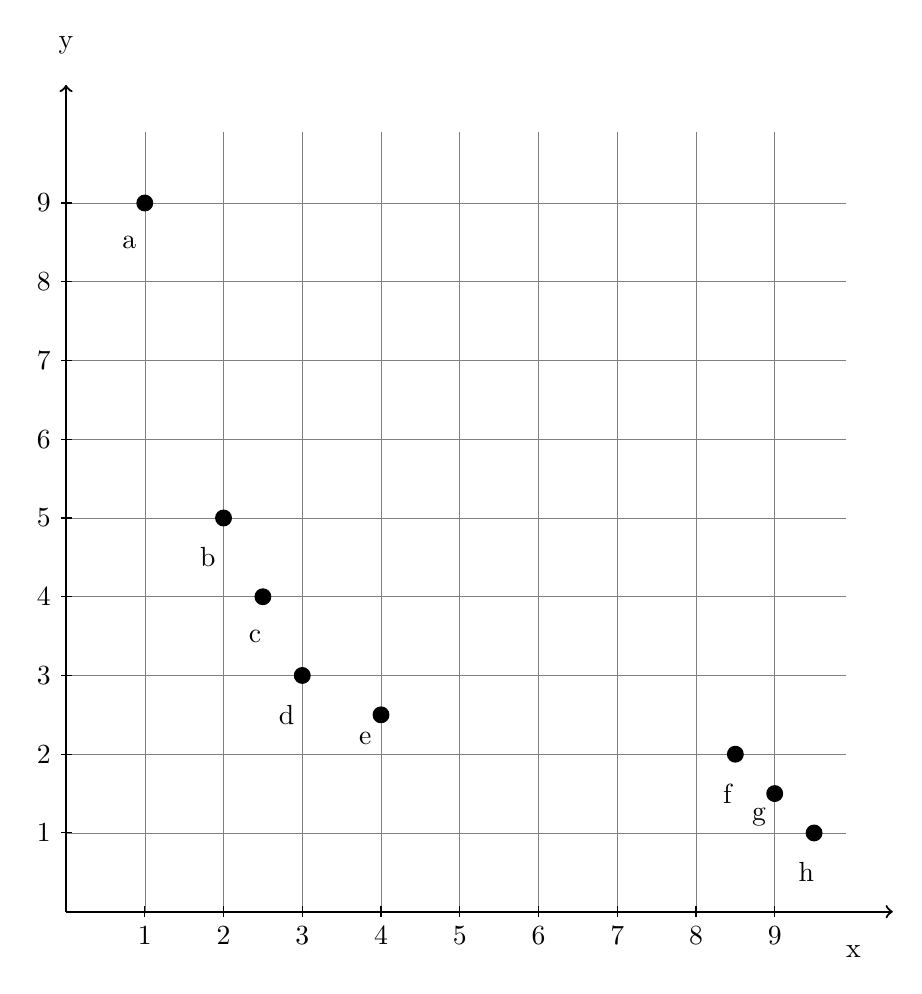
\begin{tikzpicture}
	   \draw[style=help lines] (0,0) grid (9.9,9.9)
       [step=1cm]      (1,2) grid +(1,1);
       
        \foreach \x/\xtext in {1/1,2/2,3/3,4/4,5/5,6/6,7/7,8/8,9/9}
        \draw[shift={(\x,0)}] (0pt,2pt) -- (0pt,-2pt) node[below] {$\xtext$};

		 \foreach \y/\ytext in {1/1,2/2,3/3,4/4,5/5,6/6,7/7,8/8,9/9}
         \draw[shift={(0,\y)}] (2pt,0pt) -- (-2pt,0pt) node[left] {$\ytext$};        
        
        % 4x4 grid
        \draw (0, 0) grid (10, 0);
        % x-axis
        \draw [thick,->] (0, 0) -- (10.5, 0);
        % y-axis
        \draw [thick,->] (0, 0) -- (0, 10.5);
       	%a
        \draw [color=black, fill=black] (1, 9) circle (0.1);
        \node at (0.8, 8.5) {a};
        	%b
        \draw [color=black, fill=black] (2, 5) circle (0.1);
        \node at (1.8, 4.5) {b};
        	%c
        \draw [color=black, fill=black] (2.5, 4) circle (0.1);
        \node at (2.4, 3.5) {c};
        	%d
        \draw [color=black, fill=black] (3, 3) circle (0.1);
        \node at (2.8, 2.5) {d};
        	%e
        \draw [color=black, fill=black] (4, 2.5) circle (0.1);
        \node at (3.8, 2.2) {e};
        	%f
        \draw [color=black, fill=black] (8.5, 2) circle (0.1);
        \node at (8.4, 1.5) {f};
        	%g
        \draw [color=black, fill=black] (9, 1.5) circle (0.1);
        \node at (8.8, 1.2) {g};
        	%h
        \draw [color=black, fill=black] (9.5, 1) circle (0.1);
        \node at (9.4, 0.5) {h};
        % x-axis label
        \node at (10, -0.5) {x};
        % y-axis label
        \node at (0, 11) {y};
    \end{tikzpicture}
	\caption{Beispiel einer Skyline mit zwei Dimensionen}
	\label{img:diversitaetExample}
\end{figure}

Basierend auf dem Diversitätkriterium sind in Abbildung \ref{img:diversitaetExample} drei Punkte/Datensätze am besten geeignet für die repräsentative Skyline. Punkt $a$ repräsentiert sich am besten selber. Die Punkte $b,c,d,e$ werden am besten durch $c$ oder $d$ repräsentiert, da diese relativ mittig von dieser Menge liegen. Für die restlichen Punkte ist $g$ der geeignetste.
An diesem Beispiel ist zu erkennen, dass $k$ ein wichtiger Faktor ist, um eine hohe Repräsentationsgüte zu erreichen. Denn in diesem Beispiel ist der optimale Wert von $k$ drei und ein höherer Wert würde keinen Mehrwert bzw. keine deutlich höhere Repräsentationsgüte liefern da für $k=3$ jedes Cluster einen Repräsentant hat.
%% ==============================
\section{Präferenzen}
\label{ch:Grundlagen:sec:präferenzen}
%% ==============================
Anfragen an Suchmaschinen und Datenbanken haben oft das Problem, dass sie entweder einen \enquote{empty-result} Effekt (keine Ergebnisse) oder einen \enquote{flooding-effect} (zu viele Ergebnisse) liefern. Dies frustriert in vielen Fällen den User.
Um diesem Problem zu entgehen, wurde die Standard SQL-Sprache um Präferenzen erweitert. Die Idee dahinter ist, dass der User für ihn intuitive Präferenzen (z.B. ein Auto sollte nicht mehr als 16000 \euro{} kosten) erstellen kann. Anhand dieser Präferenzen werden daraufhin die besten Ergebnisse ausgesucht.

\begin{figure}[H]
\centering
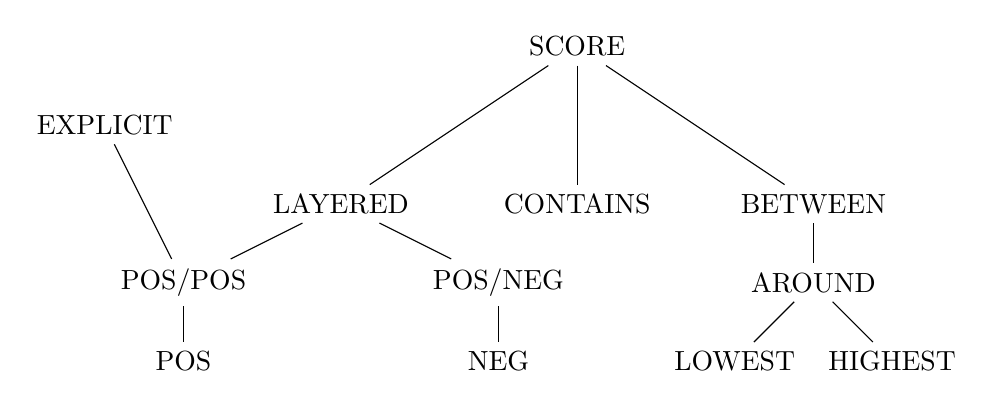
\begin{tikzpicture}
    \node (SCORE) at (0,0) {SCORE};
    \node (EXPLICIT) at (-6,-1) {EXPLICIT};
    \node (LAYERED) at (-3,-2) {LAYERED};
    \node (CONTAINS) at (0,-2) {CONTAINS};
    \node (BETWEEN) at (3,-2) {BETWEEN};
    \node (POS/POS) at (-5,-3) {POS/POS};
    \node (POS/NEG) at (-1,-3) {POS/NEG};
    \node (AROUND) at (3,-3) {AROUND};
    \node (POS) at (-5,-4) {POS};
    \node (NEG) at (-1,-4) {NEG};
    \node (LOWEST) at (2,-4) {LOWEST};
    \node (HIGHEST) at (4,-4) {HIGHEST};
    \path [-] (EXPLICIT) edge node {} (POS/POS);
    \path [-] (POS/POS) edge node {} (POS);
    \path [-] (LAYERED) edge node {} (POS/POS);
    \path [-] (LAYERED) edge node {} (POS/NEG);
    \path [-] (POS/NEG) edge node {} (NEG);
    \path [-] (SCORE) edge node {} (LAYERED);
    \path [-] (SCORE) edge node {} (CONTAINS);
    \path [-] (SCORE) edge node {} (BETWEEN);
    \path [-] (BETWEEN) edge node {} (AROUND);
    \path [-] (AROUND) edge node {} (LOWEST);
    \path [-] (AROUND) edge node {} (HIGHEST);

\end{tikzpicture}
	\caption{Beispiel einer Skyline mit zwei Dimensionen}
	\label{img:preferences}
\end{figure} 

Abbildung \ref{img:preferences} gibt einen Überblick über alle Präferenzen in Preference-SQL. In dieser Arbeit werden nur die Basispräferenzen vorgestellt, die in KNIME implementiert wurden. Die BETWEEN Präferenz erlaubt es Werte einer Dimension in einem vom User bestimmten Intervall zu präferieren. Dagegen präferiert die AROUND Präferenz Datensätze, die nah an einem bestimmten Wert liegen. Mit der LAYERED Präferenz ist es möglich Werte einer Dimension nach Wichtigkeit zu sortieren. Für Autofarben könnte folgende Reihenfolge erstellt werden: grün > schwarz > others > rot. Diese Präferenz würde als erstes grüne, darauf folgend schwarze, danach alle anderen Autos und schlussendlich rote Autos präferieren.
Die LOWEST Präferenz (Werte sollen so klein wie möglich sein) und dessen Gegenstück HIGHEST sind auch in KNIME eingebunden worden, damit Standard Skylineabfragen wie Minimum und Maximum möglich sind.
Als Zusatz wurde eine BOOLEAN Präferenz hinzugefügt, die aus dem Preference-SQL Konzept von EXASolution entnommen wurde. (vgl. \cite{EXASolution}) Hier kann der User SQL Statements eingeben, die als boolische Ausdrücke gewertet werden. Alle Datensätze, die mit diesem Ausdruck übereinstimmen und dadurch $true$ ergeben, werden bevorzugt. Im Fall des Autobeispiels könnte dies wie folgt aussehen: $price < 16000$. Mit diesem Ausdruck würden alle Autos bevorzugt, die weniger als 16000 \euro{} kosten. Dabei macht es keinen Unterschied wie niedrig der Preis ist. Alle Autos unter 16000 \euro{} werden als gleich wichtig gesehen. 

Die einzelnen Basispräferenzen können weiterhin noch mit Pareto ('AND') oder Priorisierungs ('PRIOR TO') Präferenzen verknüpft werden. Pareto verknüpfte Präferenzen haben die gleiche Wichtigkeit, wobei dazu im Gegensatz Basispräferenzen mit einer Priorisierungsverknüpfung unterschiedliche Wichtigkeit besitzen. Hierbei ist die erst genannte Basispräferenz immer wichtiger als die zweite.  

Zusätzlich zu den Verknüpfungen oder auch komplexen Präferenzen genannt, gibt es das Best Matches Only Query Model. Durch dieses Model werden \enquote{emty-results} und \enquote{flooding-effects} gemieden, da es nur die besten Ergebnisse, die sich untereinander nicht dominieren, ausgibt. Durch die Dominanz werden schlechtere Datensätze nicht zur Ergebnismenge hinzugefügt und somit wird die Anzahl der Datensätze im Ergebnis reduziert. Falls keine Datensätze vorhanden sind, die die Präferenzen optimal berücksichtigen, werden die Nächstbesten als Ergebnis genommen. Dies führt dazu, dass die Ergebnisse immer die Präferenzen so gut wie möglich berücksichtigen und die Ergebnismenge nie leer sein kann.

In Abbildung \ref{img:prefSQLSyntax} ist die Syntax zu Preference-SQL zu sehen. Hier können nach der PREFERRING Klausel die Basispräferenzen mit genannten Verknüpfungen angegeben werden. Zusätzlich kann sortiert (GROUP BY) und eine Constraint (BUT ONLY),die den \enquote{flooding-effect} noch weiter reduziert, angegeben werden. Näheres dazu kann in den diesbezüglichen Paper (\cite{kiessling2011preference}, \cite{kiessling2002foundations} und \cite{kiessling2002preference}) gelesen werden.

\begin{figure}[H]
\centering
$\begin{matrix*}[l]
\text{SELECT} & \ldots & \text{<selection>} \\
\text{FROM} & \ldots & \text{<table\char`_reference>} \\
\text{WHERE} & \ldots & \text{<hard\char`_conditions>} \\
\hspace{10pt} \textbf{PREFERRING} & \ldots & \text{<soft\char`_conditions>} \\
\hspace{10pt} \textbf{GROUPING} & \ldots & \text{<attribute\char`_list>} \\
\hspace{10pt} \textbf{BUT ONLY} & \ldots & \text{<but\char`_only\char`_condition>} \\
\text{GROUP BY} & \ldots & \text{<attribute\char`_list>} \\
\text{HAVING} & \ldots & \text{<hard\char`_conditions>} \\
\text{ORDER BY} & \ldots & \text{<attribute\char`_list>} \\
\end{matrix*}$
	\caption{Syntax von Preference-SQL}
	\label{img:prefSQLSyntax}
\end{figure} 

Zum Schluss dieses Abschnittes wird die Syntax an einem Beispiel erklärt.
Angenommen es werden alle Autos mit der höchsten PS Leistung und dem geringsten Preis gesucht. Zusätzlich sollte die Kilometeranzahl um den Wert 100000 liegen, was jedoch nicht so wichtig ist wie der Preis.
Daraus entsteht folgender Query:
\begin{verbatim}
SELECT * 
FROM car 
PREFERRING (price LOWEST PRIOR TO mileage AROUND 100000) AND
horsepower HIGHEST
\end{verbatim}


Anhand dieses Queries kann mit dem Preference-SQL JDBC Präferenzabfragen an eine Datenbank geschickt werden.
%% ==============================
\section{KNIME}
\label{ch:Grundlagen:sec:knime}
%% ==============================
KNIME oder der Konstanz Information Miner ist eine modulare Umgebung, die einen einfachen visuellen Zusammenbau und eine interaktive Ausführung von einer Data Pipeline ermöglicht. Es wird damit geworben, dass es \enquote{easy and intuitive to use} ist und \enquote{enables the user to visually explore the results} \cite[p. 2]{BCDG+07}. 

Der Konstanz Information Miner ist in Java geschrieben und dessen graphischer Workflow Editor ist als ein Eclipse Plug-in implementiert worden. Mit einer offenen API und einem Datenabstraktions Framework wird dem User erlaubt schnell Nodes zu implementieren und diese einem Workflow hinzuzufügen.

Die Architektur von KNIME unterliegt drei Prinzipien. Einem visuellen und interaktivem Framework, welches dem User ermöglicht durch einfaches Drag \& Drop Datenflüsse zu kombinieren und somit verschiedene Node Outputs als Input für andere Nodes verwenden zu können. Modularität sorgt dafür, dass alles unabhängig voneinander funktioniert. Seien es Prozesseinheiten oder Datencontainer. Dies ermöglicht eine unabhängige Implementierung von verschiedenen Algorithmen. Das letzte Prinzip ist die einfache Erweiterbarkeit. Entwickler können auf die öffentliche API zugreifen und durch das Eclipse Plug-In-Schema ohne Probleme neue Nodes entwickeln. (vgl. \cite{BCDG+07})

KNIME ermöglicht neue Algorithmen oder Visualisierungen als Nodes in KNIME zu integrieren. Nodes besitzen In- und Output Ports, die den Ein- und Ausgaben des darunter liegenden Algorithmus entsprechen. Nodes bestehen hauptsächlich aus drei Teilen: NodeModel, NodeDialog und NodeView. Das NodeModel ist dafür zuständig, dass der Algorithmus ausgeführt wird und wichtige Einstellungen gespeichert werden. Es testet, ob mit den Eingabe des Nodes der Algorithmus korrekt durchgeführt werden kann und gibt die Ergebnisse des Algorithmus aus. 
Der NodeDialog ermöglicht es dem User bestimmte Einstellungen für den Algorithmus vorzunehmen. Hierbei kann eine eigene GUI geschrieben werden oder die von KNIME vorliegenden Standardkomponenten verwendet werden. Die Kommunikation zwischen dem NodeModel und dem NodeView erfolgt durch eine Speicherung von SettingsModels in ein NodeSettings Objekt, welches von beiden Klassen geladen und gespeichert werden kann. 
Das NodeView Objekt erstellt eine graphische Darstellung der Ergebnisse des Algorithmus. Dies kann ein Histogramm, Koordinatensystem oder ähnliches sein. Die Daten für diesen View müssen vom NodeModel in einer Datei gespeichert werden, um diesen View beim Wiederöffnen von KNIME neu zu erstellen. Dies ist erforderlich, sodass zu jeder Zeit der View betrachtet werden kann und dies nicht nur nach Ausführung des Nodes möglich ist.

Workflows sind Graphen in KNIME, genau genommen gerichtete azyklische Graphen. Der dazugehörige WorkflowManager verhilft es dem User neue Nodes zum Workflow und Verbindungen zwischen den Nodes hinzuzufügen.

\begin{figure}[H]
	\centering
	\includegraphics[scale=0.8]{workflowExample.png}
	\caption{Beispiel Workflow in KNIME}
	\label{img:workflowExample}
\end{figure}

In der Abbildung \ref{img:workflowExample} ist ein Beispiel eines Workflows zu erkennen. Mit dem \textit{SQLite Connector} Node kann eine SQLite Datenbankdatei auf dem Rechner ausgewählt werden und eine Verbindung zu dieser Datenbank aufgebaut werden. Diese Verbindung wird an die anderen Nodes als Input geschickt. Für den \textit{Database Table Selector} als auch den \textit{Database Reader} Node muss eine SQL-Query im NodeDialog eingegeben werden. Der \textit{Database Table Selector} gibt eine Datenbankverbindung mit dem entsprechenden Query zurück. Im Gegensatz dazu gibt der \textit{Database Reader} Node eine Tabelle zurück, die durch die SQL Abfrage an die Datenbank entsteht. Diese Datentabellen werden in KNIME BufferedDataTables genannt. 

Da nun Preference-SQL und KNIME genauer erklärt wurden, können im nächsten Kapitel die implementieren Algorithmen vorgestellt werden.
%% ==============================
%%% End:   % Grundlagen
%% analyse.tex
\chapter{Konzept}
\label{ch:Konzept}
%% ==============================
Dieses Kapitel befasst sich darum, welche Algorithmen in KNIME implementiert wurden und erklärt deren Vorgehensweise. Zuerst wird der Block Nested Loop \cite{borzsony2001skyline}, ein Skylinealgorithmus gezeigt. Die Skyline wird von manchen repräsentativen Skylinealgorithmen zur Berechnung benötigt. Daher ist mindestens ein Skylinealgorithmus für die Arbeit zwingend notwendig. Zur Bestimmung von repräsentativen Skylines wird in dieser Arbeit als erstes der DominationMaximizer \cite{4221657} vorgestellt. Dieser versucht die \textit{k} Skylinedatensätze heraus zu suchen, die die Anzahl der dominierten Datensätze maximieren. Der zweite vorgestellte Algorithmus basiert auf Distanz \cite{Tao:2009:DRS:1546683.1547325} und sucht die Repräsentanten heraus, sodass die Distanz zwischen einem Nicht-Repräsentanten und dem nächstliegendsten Repräsentanten minimal ist. Der letzte vorgestellte Algorithmus ist der E-Greedy \cite{magnani2014taking}. Das Ziel dieses ist es die repräsentative Skyline durch Berücksichtigung von Diversität und Signifikanz der Datensätze zu bestimmen.
Zum Schluss dieses Kapitels werden genauere Details zur Funktionsweise der drei wichtigen Klassen NodeModel, NodeDialog und NodeView von KNIME aufgeführt, die für die Implementierung der Algorithmen eine wichtige Rolle spielen.
%% ==============================
\section{Block Nested Loop}
\label{ch:Analyse:sec:skyAlgos}
%% ==============================
Methoden zur Berechnung einer Skyline gibt es viele, wie zum Beispiel Nested SQL Statements, Block-Nested-Loop, Divide \& Conquer, etc.
Zusätzlich gibt es auch viele Ansätze, die auf B/R-Bäume aufbauen, wie zum Beispiel der Algorithmus in \cite{Papadias:2003:OPA:872757.872814}. Der Vorteil bei diesen ist, dass sie während der Berechnung schon Datensätze der Skyline ausgeben können und im Fall von Suchabfragen dem User schon nach kurzer Zeit einige Ergebnisse liefern können. Weiterhin sind Algorithmen, die auf B/R-Bäumen basieren oft schneller als andere Algorithmen, da oft viele Vergleiche durch Pruning der Bäume oder mithilfe der Branch \& Bound Methode reduziert werden können. 
Da in dieser Arbeit der Mittelpunkt repräsentative Skyline sind, wurde für diese Arbeit nur der Block-Nested-Loop Algorithmus implementiert, da dieser intuitiv und für den Zweck dieser Arbeit ausreichend ist. Weitere Skyline-Algorithmen in KNIME einzubauen, wäre ein guter Schritt diese Arbeit fortzusetzen. 

Der Block-Nested-Loop Algorithmus basiert auf einer einfachen geschachtelten Schleife. Zur Reduzierung der Rechenzeit wurde ein Fenster $w$ eingeführt, in welchem unvergleichbare bzw. undominierte Datensätze gespeichert werden. Meistens bestimmt der User wie viele Datensätze im Fenster gespeichert werden können.
Beim Einlesen eines Datensatzes, wird er mit allen anderen Datensätzen in $w$ verglichen. Hier gibt es drei Möglichkeiten:
Falls der eingelesene Datensatz $p$ von einem oder mehreren Datensätzen in $w$ dominiert wird, wird er eliminiert und in folgenden Iterationen nicht mehr betrachtet. Dies führt zu großen Einsparungen der Rechenzeit. 
Falls $p$ jedoch einen oder mehrere Datensätze in $w$ dominiert, werden diese Datensätze von $w$ entfernt und $p$ wird zu $w$ hinzugefügt.
Bei Unvergleichbarkeit wird $p$ in $w$ eingefügt, falls in $w$ noch nicht die vom User bestimmte Grenze erreicht ist. Ansonsten wird $p$ in eine temporäre Datei geschrieben.

Die Datensätze in der temporären Datei werden in der nächsten Iteration mit dem Fenster verglichen. Dieser Vorgang wird so lange wiederholt bis nach einer Iteration kein Datensatz mehr in der temporären Datei vorhanden ist.
Damit dieser Vorgang terminiert, bekommen Datensätze beim Einfügen in $w$ oder in die temporäre Datei einen Zeitstempel. Beim Einlesen des Datensatzes, wird jeder Datensatz in $w$ mit einem geringeren Zeitstempel ausgegeben  bzw. in die Skyline eingefügt.
Weiterhin werden nach der ersten Iteration alle Datensätze aus $w$ zur Skyline hinzugefügt, bei der während des Hinzufügens in $w$ die temporäre Datei leer war.
Diese beiden Kriterien sorgen nicht nur für die sichere Terminierung des Algorithmus, sondern auch für eine Einsparung der Rechenzeit.
Ein Pseudo-Code für diesen Algorithmus befindet sich im Anhang von \cite{borzsony2001skyline}.

Da sich diese Arbeit hauptsächlich um repräsentative Skylines und Präferenzen befasst und trotzdem eine Implementierung eines Skylinealgorithmus erforderlich war, fiel die Entscheidung auf den Block-Nested-Loop. Dieser war einfach und schnell zu implementieren und liefert im Gegensatz zu einer normalen verschachtelten Schleife ein schnelleres Ergebnis.  
%% ==============================
\section{Repräsentative Skyline Algorithmen}
\label{ch:Analyse:sec:repSkyAlgos}
%% ==============================
In diesem Abschnitt des Kapitels werden die Algorithmen zur Berechnung einer repräsentativen Skyline, die für diese Arbeit in KNIME implementiert wurden, vorgestellt. 
Diese basieren hauptsächlich auf einen der zwei Ziele: Diversität oder Signifikanz zu maximieren (siehe Abschnitt \ref{ch:Grundlagen:sec:repSkyline}).
Zur Gegenüberstellung wurden sowohl Algorithmen implementiert, die den originalen Datensatz als Eingabe bekommen als auch welche, die nur mit einer Skyline als Eingabe arbeiten können.
%% ==============================
\subsection{DominationMaximizer}
\label{ch:Analyse:sec:repSkyAlgos:subsec:domMax}
%% ==============================
Der DominationMaximizer (Algorithmus \ref{algo:domMaximizer}) ist eine kleine Abwandlung des Greedy-Algorithmus, der in Kapitel 5.2 von \cite{4221657} vorgestellt wird. 
Das Ziel beider Algorithmen ist es $k$ Datensätze zu finden, die zusammen maximal viel andere Datensätze dominieren.

\begin{algorithm}[H]
\caption{DominationMaximizer}\label{algo:domMaximizer}
\begin{algorithmic}[1]
\INPUTBF $k$ int, $P$ set of data points
\OUTPUTBF $k$ skyline points
\State $S_P = \varnothing$ and $S = \varnothing$
\State \textbf{for each} data point $p$ in $P$ 
\State \hspace{\algorithmicindent} \textbf{for each} data point $q$ in $P$
\State \hspace{\algorithmicindent} \hspace{\algorithmicindent} \textbf{if} $p \succ q$ \textbf{then} 
\State \hspace{\algorithmicindent} \hspace{\algorithmicindent} \hspace{\algorithmicindent} $S_P:= S_P \cup \{p\}$ and $S_P:= S_P-\{q\}$
\State \hspace{\algorithmicindent} \hspace{\algorithmicindent} \hspace{\algorithmicindent} $D(\{p\}):=D(\{p\}) \cup \{q\}$  
\State \textbf{while} $|S|<k$ and $S_P-S \neq \varnothing$ \textbf{do}
\State \hspace{\algorithmicindent} choose $s \in {S_P-S}$ such that $|D(\{s\} \cup S)|$ is maximized
\State \hspace{\algorithmicindent} $S:=\{s\} \cup S$
\State \textbf{return} $S$
\end{algorithmic}
\end{algorithm}

Im Gegensatz zum Greedy-Algorithmus berechnet der DominationMaximizer Algorithmus die Skyline und die Menge der dominierten Datensätze für jeden undominierten Datensatz gleichzeitig. Falls bei einem Vergleich zwischen zwei Datensätzen einer der beiden vom anderen dominiert wird, wird der dominierte Datensatz der Menge $D$ des dominierenden Datensatzes hinzugefügt. $D\{s\}$ ist somit die Menge von Datensätzen, die von Datensatz $s$ dominiert werden. 

Der Greedy-Algorithmus legt nicht fest, welcher Algorithmus für die Berechnung der Skyline benötigt wird. Für den DominationMaximizer wird eine einfache verschachtelte Schleife verwendet, um sicher zu stellen, dass jeder Datensatz mit allen anderen verglichen wird. 
Nach dem Durchlaufen der Schleife werden $k$ Datensätze ausgewählt, die erstens von keinem anderen Datensatz dominiert werden und die die Menge an dominierten Datensätzen maximieren.

Das Problem dieses Algorithmus ist, dass bei Daten mit geringer Streuung und wenigen vorhandenen Ausreißer nur Skylinedatensätze, die nah an dominierten Datensätzen liegen, in der repräsentativen Skyline enthalten sind. Dies liegt daran, dass Skylinedatensätze, die nah an dominierten Datensätzen liegen, sehr wahrscheinlich in allen betrachteten Dimensionen besser sind als die dominierten und somit am meisten Datensätze dominieren.  Da Ausreißer meistens nur undominierten Datensätzen entsprechen, die keinen anderen Datensatz dominieren, werden diese meistens vom DominationMaximizer nicht zur Skyline hinzugefügt. Dies hat zur Folge, dass die Repräsentationsgüte für solche Fälle relativ niedrig ist, da Ausreißer dadurch nie in der repräsentativen Skyline enthalten sind, was gut in Abbildung \ref{img:dominationMaximizerGraph} zu sehen ist.
 
\begin{figure}[H]
	\centering
	\includegraphics[width=\textwidth]{dominationMaximizerGraph.png}
	\caption{Die repräsentative Skyline des DominationMaximizer bei Daten mit hoher Dichte}
	\label{img:dominationMaximizerGraph}
\end{figure}
%% ==============================
\subsection{Distanz-basierende repräsentative Skyline}
\label{ch:Analyse:sec:repSkyAlgos:subsec:disBasedRepSky}
%% ==============================
Angenommen die Menge $S$ beinhaltet alle Skylinedatensätze und $K$ entspricht einer repräsentativen Skyline mit $k$ Datensätzen. Mit diesen beiden Mengen kann nun der repräsentative Fehler $Er(K,S)$ berechnet werden. 
$$Er(K,S)=\max\limits_{p\in{S-K}}\{\min\limits_{p^{'} \in{K}}||p,p^{'}||\}$$
Entsprechend dieses Fehlers ist eine repräsentative Skyline gut, falls für jeden nicht repräsentativen $\in{S-K}$, ein repräsentativer $\in{K}$ in der Nähe ist. An der Formel ist zu erkennen, dass der Fehler die Repräsentationsgüte anhand der Distanz zwischen einem nicht-repräsentativen Datensatz und dem nächstliegenden repräsentativen Datensatz misst. Diese Distanz wird mit der euklidischen Distanz berechnet.
Das Ziel des Algorithmus ist es die $k$ Datensätze zu finden, mit denen dieser repräsentative Fehler minimal ist. Bedingung für die korrekte Durchführung des Algorithmus sind, dass alle Datensätze nur zwei Dimensionen besitzen oder nur zwei betrachtet werden. Zusätzlich sollten die Datensätze nach der ersten Dimension aufsteigend sortiert werden. Für dieses Arbeit wird der Algorithmus in KNIME implementiert und dadurch wird die Sortierung im entsprechenden KNIME Node durchgeführt, damit sich der User damit nicht befassen muss. 

Die Funktion $opt(i,t)$ bestimmt die $t$ große optimale repräsentative Skyline von $S_i$, wobei $t \leq i$ gilt. $S_i$ ist hier eine Teilmenge von $S$ mit $i \leq m$ (m=Anzahl der Skylinedatensätze). Falls $i=m$ und somit $S_i=S$ gilt, entspricht $opt(m,k)$ der optimalen $k$ großen repräsentativen Skyline von $S$.
Um diese Funktion jedoch berechnen zu können, muss zuerst der optimale Repräsentationsfehler von $opt(i,t)$ bestimmt werden.
$$optEr(i,t)=\min\limits_{j=t}^{i-1}\{max\{optEr(j-1,t-1),radius(j,i)\}\}$$
Die Werte von $i$,$j$ und $t$ entsprechen den Indizes von Datensätzen der Skyline. Diese Formel bestimmt rekursiv die $t$ kleinsten Radien beziehungsweise die $t$ kleinsten Kreise, die zusammen alle $m$ Datensätze umfassen. Es ist zu erkennen, dass der repräsentative Fehler dem niedrigsten Radius entspricht, der die meisten Datensätze umfasst.

Angenommen $v$ sei der Wert von $j$ bei dem oben genannte Funktion $optEr(i,t)$ ihr Minimum findet\footnote{Die Indizes der beiden Funktionen müssen hierbei identisch sein. Für $opt(8,3)$ wird der Wert von $j$ für $v$ verwendet, bei der die Funktion $optEr(8,3)$ ihr Minimum erreicht.}, dann ergibt sich die repräsentative Skyline durch folgende Funktion:
$$opt(i,t)=opt(v-1,t-1)\cup\{center(v,i)\}$$
Diese Funktion wird wie $optEr(i,t)$ rekursiv berechnet und fügt die Datensätze hinzu, die Mittelpunkte der Kreise sind, die alle $i$ Datensätze umfassen. Dadurch das $v$ der Wert von $j$ ist, bei der die Funktion $optEr(i,t)$ ihr Minimum erreicht, wird erzwungen das nur Kreise betrachtet werden, die mit geringem Radius die meisten Datensätze umfassen.   
Für die Berechnung der umfassenden Kreisradien, wird die euklidische Distanz benutzt:
$$radius(i,j)=\min\limits_{u=i}^{j}\{max\{||p_i,p_u||,||p_u,p_j||\}\}$$
Der Punkt $p_u=center(i,j)$ bei dem diese Funktion ihr Minimum erreicht, ist der Mittelpunkt des Kreises, der alle Datensätze zwischen den Datensätzen bei Index $i$ und $j$ umfasst.

\begin{algorithm}[H]
\caption{2D-opt ($S$,$k$)}\label{algo:2DOpt}
\begin{algorithmic}[1]
\INPUTBF the skyline $S$ of dataset $D$ and an integer $k$
\OUTPUTBF the representative skyline of $D$
\State \parbox[t]{\dimexpr\linewidth-\algorithmicindent}{\textbf{for each} pair of $(i,j)$ such that $1 \leq i \leq j \leq m$, derive\par 
$radius(i,j)$ and $center(i,j)$\strut}
\State \parbox[t]{\dimexpr\linewidth-\algorithmicindent}{set $opt(i,1) = \{center(1,i)\}$ and $optEr(i,1)=radius(1,i)$\par
\textbf{for each} $1 \leq i \leq m$\strut}
\State \textbf{for} $t=2$ \textbf{to} $k-1$
\State \hspace{\algorithmicindent} \textbf{for} $i=t$ \textbf{to} $m$
\State \hspace{\algorithmicindent}\hspace{\algorithmicindent} compute $optEr(i,t)$
\State \hspace{\algorithmicindent}\hspace{\algorithmicindent} compute $opt(i,t)$
\State compute $optEr(m,k)$ and $opt(m,k)$
\State \textbf{return} $opt(m,k)$
\end{algorithmic}
\end{algorithm}

Algorithmus \ref{algo:2DOpt} berechnet zuerst alle wichtigen Werte, die für die $k$ repräsentative Skyline mit $m$ Skylinedatensätzen benötigt wird. Zeile $2$ dient dazu, dass sowohl $opt(i,t)$ als auch $optEr(i,t)$ terminieren. Das Paper \cite{Tao:2009:DRS:1546683.1547325} dieses Algorithmus berechnet in Zeile $7$ die Funktionen $optEr(k,m)$ und $opt(k,m)$ und nicht $optEr(k,m)$ und $opt(k,m)$. Dies hätte zur Folge, dass für die Berechnung der Formeln $i$ kleiner als $t$ ist und es somit nie zu einem Ergebnis kommen würde.
Das Ergebnis von $opt(m,k)$ kann als repräsentative Skyline ausgegeben werden und dem Kunden präsentiert werden.

Der Algorithmus basiert nur auf Diversität und versucht Datensätze, die möglich weit voneinander entfernt sind zu finden, um damit alle möglichen Cluster der Skyline repräsentieren zu können. Der Algorithmus im nächsten Abschnitts versucht diesen Ansatz zu erweitern und berücksichtigt zusätzlich die Signifikanz von Datensätzen, falls diese gegeben sind.  
%% ==============================
\subsection{E-Greedy}
\label{ch:Analyse:sec:repSkyAlgos:subsec:eGreedy}
%% ==============================
Der E-Greedy Algorithmus \cite{magnani2014taking} versucht nicht nur die Diversität von Datensätzen zu maximieren, sondern auch gleichzeitig die Signifikanz zu beachten.
Signifikanz wird dadurch bestimmt, indem der User für jede Dimension seiner Wahl einen Thresholdwert oder ein Thresholdintervall angibt. Die Datensätze, die entweder den Thresholdwert übersteigen bzw. unter diesem liegen oder in dem entsprechenden Intervall liegen, sind signifikant. Bei fehlenden Thresholds einer Dimension werden alle Datensätze bei alleiniger Betrachtung dieser Dimension als gleich signifikant gesehen. Dieser Ansatz kann noch erweitert werden, indem Thresholds durch vergangene Daten bestimmt werden. 

$$\text{Representative Skyline} = \argmax{S \in{P_k(sky(R))}} obj(S)$$

$obj(S)$ ist hier eine Funktion, die die Werte der Diversität und Signifikanz darstellt. $P_k(sky(R))$ ist eine Teilmenge mit $k$ Datensätzen der Skyline. Somit entspricht die repräsentative Skyline der Teilmenge, bei der die Funktion $obj(S)$ ihr Maximum erreicht.

$$\lambda \sum\limits_{r \in{S \backslash \{r\}}} min_{s \in S \backslash \{r\}}\delta(r,s)+(1- \lambda) \sum\limits_{r \in{S}}E(\sigma(r))$$

Die Funktion $obj(S)$ besteht aus zwei Teilen. Der Signifikanz $\sigma$ und der Diversität $\delta$.
Mit einem Gewichtungsfaktor $\lambda$ kann der User bestimmen, welcher der beiden Aspekte ihm wichtiger ist. Anzumerken ist, dass der \textbf{erwartete} Wert der Signifikanz $\sigma(r)$ berechnet wird. 

$$\begin{displaystyle}
  I_i(r, s) = \left.
  \begin{cases}
    0 & \text{if } r=s \\
    \frac{|\{o \in{sky(R)}| (r.i \geq o.i \geq s.i) \lor (s.i \geq o.i \geq r.i)\}|-1}{|sky(R)|-1} & \text{if } r \neq s
  \end{cases}
  \right.
\end{displaystyle}$$

Um die Diversität zu berechnen, wird für jede Datensatzkombination und jede Dimension $i$ die Anzahl von Skylinedatensätzen, die zwischen zwei Datensätzen liegt, gezählt. Da $I_i$ dem relativen Anteil der dazwischen liegenden Punkte entsprechen soll, wird durch die $\text{Anzahl aller Skylinedatensätze}-1$ geteilt.

$$\delta_{sed}(r,s)=\frac{\sum\limits\mathop{}_{\mkern-5mu i \in{[1,d]}} I_i(r,s)}{d}$$

Durch das Summieren aller $I_i$, geteilt durch die Anzahl der Dimensionen, entsteht schlussendlich die Diversität bzw. den Wert wie sehr die Datensätze $r$ und $s$ voneinander abweichen. Diesen Wert zu maximieren führt dazu, dass die Anzahl der Datensätze zwischen zwei Datensätzen maximal sein sollte. Dadurch enthält die repräsentative Skyline bei alleiniger Betrachtung von Diversität nur Datensätze, die weit voneinander entfernt sind. 

$$\sigma_{sss}(r)=\frac{logit(r)}{max\mathop{}_{\mkern-5mu s \in{sky(R)}}logit(s)}$$

Da die Thresholds durch einen User bestimmt werden, wird die für die Berücksichtigung der Signifikanz die Sigmoid Funktion benutzt, da diese User Präferenzen repräsentieren kann. Die Skyline Sigmoid Signifikanz $\sigma_{sss}$ ergibt sich durch die logistische Sigmoid Funktion des betrachteten Datensatzes geteilt durch die logistische Sigmoid Funktion des Datensatzes, der von allen Datensätzen den höchsten Wert für die logistische Sigmoid Funktion besitzt. Die logistische Sigmoid Funktion wird je nachdem, ob der Benutzer einen einzelnen Thresholdwert oder ein Thresholdintervall eingegeben hat, anders berechnet.

Wie oben genannt wird eine Eingabe eines Thresholds für die Berechnung der Signifikanz benötigt. Bei der Eingabe eines einzelnen Wertes, hier $t$ genannt, wird die logistische Sigmoidfunktion wie folgt bestimmt:

$$logit(r)=\frac{\sum\mathop{}_{\mkern-5mu i \in{[1,d]}\frac{1}{1+e^{-r.i+t.i}}}}{d}$$

Zur Berechnung der logistischen Sigmoidfunktion  wird $\frac{1}{1+e^{-r.i+t.i}}$ für alle Dimension summiert, wobei $r.i$ der Wert von Dimension $i$ des entsprechenden Datensatzes $r$ entspricht. $t.i$ entspricht dagegen dem Wert des Thresholds für diese Dimension. Diese Funktion wird benutzt falls der Threshold als untere Grenze benutzt wird und alle Datensätze mit Werten über diesem Threshold als signifikant gesehen werden. 
Es wird angenommen, dass der User ein Auto mit einer PS-Leistung von 100 oder mehr bevorzugt. Aus dieser Angabe würde sich für $\frac{1}{1+e^{-r.i+t.i}}$ der Funktionsgraph in Abbildung \ref{img:logitFunction} ergeben. Es ist gut zu erkennen, dass bei einem Wert von 100 die Signifikanz bei $50\%$ liegt und somit bei einer reinen Betrachtung der PS-Leistung jedes Auto mit einer höheren PS-Leistung als signifikant gesehen wird.

\begin{figure}[H]
	\centering
	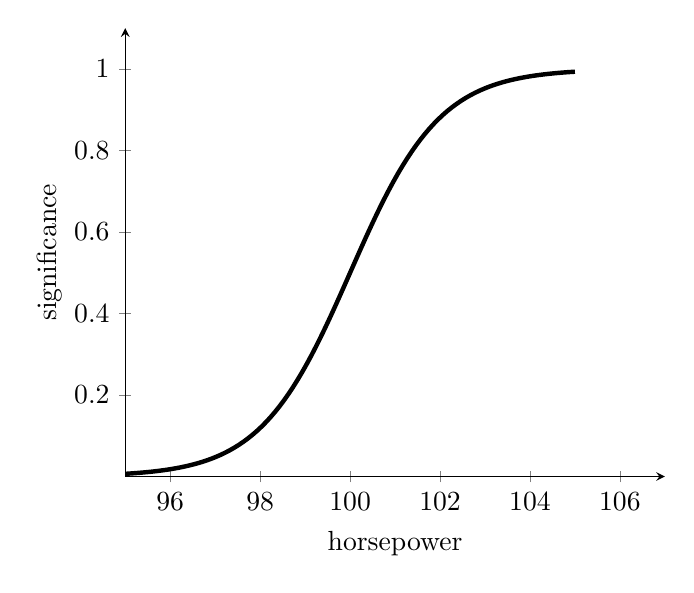
\begin{tikzpicture}
	\begin{axis}[
    axis lines=middle,
    xmax=107,
    xmin=95,
    ymin=0,
    ymax=1.1,
     x label style={at={(axis description cs:0.5,-0.1)},anchor=north},
    y label style={at={(axis description 	cs:-0.1,.5)},rotate=90,anchor=south},
    xlabel={horsepower},
    ylabel={significance}
    ]
    \addplot [domain=95:105, samples=100, ultra thick, black] {1/(1+e^(-	x+100))};
    \vasymptote {100}
	\end{axis}
\end{tikzpicture}
	\caption{Die Funktion $\frac{1}{1+e^{-r.i+t.i}}$ bei einem Thresholdwert von 100}
	\label{img:logitFunction}
\end{figure}

Falls jedoch der Threshold als obere Grenze genommen wird, ändert sich die Funktion wie folgt:

$$logit(r)=\frac{\sum\mathop{}_{\mkern-5mu i \in{[1,d]}\frac{1}{1+e^{r.i-t.i}}}}{d}$$

Für Thresholdintervalls sind diejenigen Datensätze signifikant, dessen Werte in dem Intervall liegen. Die dazugehörige Logit-Funktion wird wie folgt berechnet:
$$logit(r)=\frac{\sum\limits\mathop{}_{\mkern-5mu i \in{[1,d]}}\frac{1}{b.i-a.i}(-ln(1+e^{(r-i-b.i)})+ln(1+e^{(r.i-a.i)}))}{d}$$

$a.i$ entspricht hier der unteren Grenze und $b.i$ der obere Grenze des Thresholdintervalls. 


Nach der Berechnung der Signifikanz und der Diversität, kann die endgültige Objektfunktion bestimmt werden, die hier $\bar{\delta}$ genannt wird.
$$\bar{\delta}(r,s)= \lambda \text{ } \delta(r,s)+(1- \lambda)E(\sigma(r))$$

Um nun die $k$ repräsentativen Skylinedatensätzen zu bestimmen, die diese Objektfunktion maximieren, wird der Algorithmus \ref{algo:eGreedy} benutzt. 


\begin{algorithm}[H]
\caption{E-Greedy}\label{algo:eGreedy}
\begin{algorithmic}[1]
\INPUTBF $S$ skyline, $k$ int
\State RS $:=$ emptylist
\State RS $\leftarrow$ most significant record in $S$
\State \textbf{for} $i: 1\ldots k-1$ \textbf{do}
\State \hspace{\algorithmicindent}r = $arg$ $max_{r\in{S}}$ $\bar{\delta}(r,RS)$
\State \hspace{\algorithmicindent} RS $\leftarrow$ r
\State \textbf{end for}
\State \textbf{return} RS
\end{algorithmic}
\end{algorithm}

Der erste Datensatz der zur repräsentativen Skyline hinzugefügt wird, ist der Datensatz mit der höchsten Signifikanz. Falls mehrere die gleiche Signifikanz besitzen, wird ein Datensatz von diesen zufällig ausgewählt.
Anschließend werden $k-1$ Datensätze hinzugefügt, die mit der bereits berechneten repräsentativen Skyline die Objektfunktion maximieren.

Der Vorteil des E-Greedy liegt darin, dass er sowohl Signifikanz als auch Diversität betrachtet. Andere Ansätze zur Berechnung von repräsentativen Skylines beruhen meistens nur auf einer der beiden Kriterien.  
\enquote{Existing approaches have only focused on partial aspects of this problem. Some try to identify sets of diverse records giving an overall approximation of the skyline. [...] Others exploit some knowledge of the record scoring function to identify the most significant record, but not sets of records representative of the whole skyline.} \cite[p. 1]{magnani2014taking}
 
Die Signifikanz den User bestimmen zu lassen, liefert eine repräsentative Skyline für seine Präferenzen entsprechend. Falls nun noch die Diversität betrachtet wird, können auch Ausreißer und die Verschiedenheit von Datensätzen berücksichtigt werden. Dies ermöglicht auch repräsentative Skylines zu berechnen für die der User nur bei bestimmten Dimensionen Thresholds festlegen kann.
Der Nachteil dieses Algorithmus ist, dass der Gewichtungsfaktor $\lambda$ die repräsentative Skyline stark verändert und der User oft nicht weiß wie er die Diversität und die Signifikanz gegeneinander gewichten soll. Dies bedeutet, dass es dazu kommen kann, dass die repräsentative Skyline mehr als nur einmal berechnet wird, um ein zufrieden stellendes Ergebnis zu finden.
%% ==============================
\section{KNIME}
\label{ch:Analyse:sec:knime}
%% ==============================
Wie schon in Abschnitt \ref{ch:Grundlagen:sec:knime} erwähnt, wird für die Implementierung KNIME benutzt. Ein Node in KNIME besteht aus mehreren wichtigen Klassen, die in diesem Kapitel vorgestellt werden.
%% ==============================
\subsection{NodeModel}
\label{ch:Analyse:sec:knime:subsec:nodeModel}
%% ==============================
Das NodeModel ist dafür zuständig den Algorithmus auszuführen und wichtige Daten intern zu speichern. 
Weiterhin wird überprüft, ob die Eingaben des Nodes die korrekten Datentypen besitzen und nicht leer sind.
Eingaben können zum Beispiel Datenbankverbindungen oder Datentabellen, in KNIME BufferedDataTables genannt, sein. Falls die Eingaben inkorrekt sind, kann eine Exception geworfen werden, die dem User einen Fehler anzeigt (siehe \ref{img:nodeModelError}).

\begin{figure}[H]
	\centering
	\includegraphics[width=\textwidth]{nodeModelError.png}
	\caption{Fehleranzeige eines Nodes}
	\label{img:nodeModelError}
\end{figure}

Es kann zusätzlich überprüft werden, ob mit den Eingaben der Algorithmus des Nodes durchführbar ist. Falls ein Algorithmus nur mit numerischen Werten arbeitet, kann überprüft werden, ob einzelne Datenspalten eines BufferedDataTables nur numerische Daten enthalten.

Nach Überprüfung der Eingaben werden diese dem auszuführenden Algorithmus übergeben, der daraufhin entsprechende Ausgaben zurück gibt. Weiterhin werden im NodeModel Meta Informationen zu den Ausgaben erstellt, um einen schnellen Zugriff auf Informationen wie Datenspaltennamen zu gewährleisten.

NodeModels können SettingsModels besitzen, die die Eingaben des Users im NodeDialog speichern. Die Wert dieser SettingsModels können für den Algorithmus oder dem NodeView verwendet werden. Das NodeModel besitzt auch Methoden, die zur Speicherung bestimmter Variablen und der genannten SettingModels benötigt werden, um diese beim Wiederöffnen von KNIME zu laden.
%% ==============================
\subsection{NodeDialog}
\label{ch:Analyse:sec:knime:subsec:nodeDialog}
%% ==============================
Diese Klasse dient dazu dem User eine Möglichkeit zu bieten, bestimmte Parameter für den Algorithmus selbst einstellen zu können. 
Dazu können entweder Standardkomponenten von KNIME verwendet werden oder es wird eine eigene graphische Oberfläche dem NodeDialog hinzugefügt.

Um diese Parameter der NodeModel Klasse und somit dem Algorithmus zu übergeben, werden die vorher erwähnten SettingModels benutzt. Diese können mit einem speziellen Schlüssel im NodeModel geladen werden.
Es können aber auch Variablen mit primitiven Datentypen durch die entsprechenden Methoden des NodeDialogs gespeichert und daraufhin im NodeModel zugegriffen werden.

In Abbildung \ref{img:nodeDialog} ist ein Beispiel des NodeDialogs des Database Connector Nodes zu sehen, für den eine Datenbank URL, ein JDBC Treiber und weitere Eingaben eingegeben werden können, um eine Datenbankverbindung aufzubauen.

\begin{figure}[H]
	\centering
	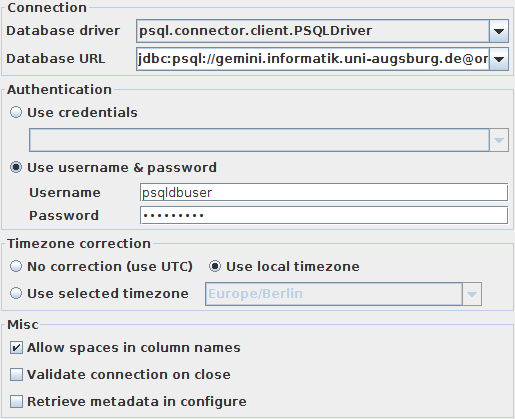
\includegraphics{nodeDialog.png}
	\caption{NodeDialogs des Database Connector Nodes}
	\label{img:nodeDialog}
\end{figure}

%% ==============================
\subsection{NodeView}
\label{ch:Analyse:sec:knime:subsec:nodeView}
%% ==============================
Die letzte Klasse, die von großer Relevanz ist, erzeugt eine Darstellung der Ein- oder Ausgaben. Die Darstellung kann je nach Ein- oder Ausgaben variieren (Histogramme, Koordinatensysteme mit Datenpunkten, Pie Charts, etc.).
Da der View eines Nodes nicht gespeichert wird, muss er bei jedem Öffnen von KNIME neu erzeugt werden.
Deswegen gibt es Methoden im NodeModel, die die Daten, die zur Erzeugung des Views benötigt werden in einer externen Datei speichern. Wie die SettingModels werden interne Dateien mit einem speziellen Schlüssel gespeichert und geladen. Im Gegensatz zur Kommunikation zwischen NodeModel und NodeDialog ist es möglich im NodeView durch Getter Methoden auf die Variablen der NodeModel Klasse zurückzugreifen. 

In Abbildung \ref{img:nodeView} ist ein Beispiel View des Histogramm Nodes zu sehen, der als Eingabe einen BufferedDataTable bekommt und nach Auswahl bestimmter Dimensionen ein Histogramm zeigt. 

\begin{figure}[H]
	\centering
	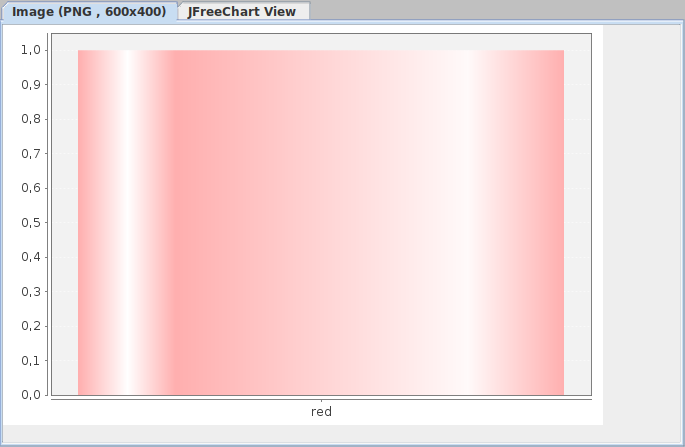
\includegraphics[width=\textwidth]{nodeView.png}
	\caption{Beispiel View des Histogramm Nodes}
	\label{img:nodeView}
\end{figure}

Nähere Informationen zur Funktionsweise und Implementierung von Nodes können auf der Webseite\footnote{https://tech.knime.org/developers (28.10.2016)} und dem Paper \cite{BCDG+07} von KNIME gefunden werden.
%% ==============================
%%% End: 
     % Analyse
%% implemen.tex
\chapter{Implementierung}
\label{ch:Implementierung}
%% ==============================
Dieses Kapitel befasst sich mit der Implementierung der Algorithmen aus Kapitel \ref{ch:Grundlagen}. Zuerst werden jeweils die Ein- und Ausgaben der verschiedenen Nodes, deren Nutzen und Funktionsweise erklärt. 
Danach werden die einzelnen Schritte der Implementierung des NodeDialogs und NodeModels erläutert. Falls eine Implementierung eines Views vorhanden ist, wird diese auch präsentiert.
%% ==============================
\section{PreferenceCreator Node}
\label{ch:Implementierung:sec:prefCreatorNode}
%% ==============================
\begin{figure}[H]
	\centering
	\includegraphics[width=0.23\textwidth]{prefCreatorLogo.png}
	\caption{PreferenceCreator Node}
	\label{img:prefCreatorLogo}
\end{figure} 

In Figur \ref{img:prefCreatorLogo} ist der PreferenceCreator Node zu sehen. Dieser nimmt als Eingabe ein DatabasePortObject und einen BufferedDataTable an. Das DatabasePortObject enthält den Typ der Datenbankverbindung, einen SQL-Query und die entsprechende Verbindung mit Datenbank-URL und JDBC Treiber. Zusätzlich enthält das Objekt auch einen Usernamen und das dazugehörige Passwort, falls dies für die Datenbank Authentifizierung notwendig ist. Mit Hilfe des Querys und der Verbindung können Datensätze abgerufen werden und für den Algorithmus verwendet werden. 
In Abbildung \ref{img:prefCreatorDBConnection} ist einer dieser Objekte mit allen eingegeben Daten zu sehen, wohingegen Abbildung \ref{img:prefCreatorDataTable} einem Teil der Datensätzen des BufferedDataTables entspricht. Dieser BufferedDataTable wird für den NodeDialog benötigt, um alle Dimensionen dieser Tabelle in einer Auswahlbox anzuzeigen, da im NodeDialog die Datensätze nicht mit der Datenbankverbindung abgerufen werden können. Es ist notwendig, dass mit dem Query des DatabasePortObjects der gleiche BufferedDataTable entsteht, der als Eingabe in den Node kommt, da sonst mit falschen Daten weitergearbeitet wird. Deshalb wird in der $configure$ Methode des NodeModels geprüft, ob das DatabasePortObject den gleichen BufferedDataTable zurück liefert wie der als Eingabe in diesen Node kommende BufferedDataTable. Falls dieser Test fehlschlägt, kann der Node nicht ausgeführt werden. 

\begin{figure}[H]
	\centering
	\includegraphics[width=0.85\textwidth]{prefCreatorDBConnection.png}
	\caption{DataBaseConnection Inport des PreferenceCreator Nodes}
	\label{img:prefCreatorDBConnection}
\end{figure}

\begin{figure}[H]
	\centering
	\includegraphics[width=1.0\textwidth]{prefCreatorDataTable.png}
	\caption{BufferedDataTable Inport des PreferenceCreator Nodes}
	\label{img:prefCreatorDataTable}
\end{figure}

Bei der Ausführung des Nodes werden zwei SQL-Queries erzeugt. Der Score-Query und der Preference-Query. Der Score-Query bewertet jeden Datensatz anhand der Präferenzen des Users, die im NodeDialog eingegeben werden und der Preference-Query entspricht einem Preference-SQL Query (siehe Kapitel \ref{ch:Forschungsstand:sec:prefSQL}) basierend auf den selben Präferenzen. 

Einer der Ausgaben des Nodes entspricht dem selben DataBasePortObject, welches als Eingabe in den Node kommt. Diese Ausgabe wird von nachfolgenden Nodes benutzt, um sich mit der Datenbank zu verbinden und dadurch ein Zugriff auf die originalen Daten möglich ist. Die meisten nachfolgende Nodes benutzen sowohl den Score-Query als auch den ursprünglichen Query, der als  Zusatzinformation für das DatabasePortObject enthalten ist. Der Grund dafür ist, dass die meisten Nodes dieser Arbeit sowohl die bewerteten Datensätze (Datensätze, die durch den Score-Query entstehen), als auch den Originaldatensatz benötigen. Um beides zu ermöglichen, werden der Score-Query, der Preference-Query und weitere Informationen, die später noch genannt werden, als versteckte Flowvariablen an folgende Nodes weitergegeben. Nachfolgende Nodes sind hierbei alle Nodes, die im vorhergehenden Datenfluss einen PreferenceCreator Node besitzen. Diese müssen nicht zwingend direkte Nachfolger des PreferenceCreator Nodes sein, sondern können auch Enkelkinder sein.

Wie schon erwähnt benutzen die meisten Nodes den Score-Query mit den bewerteten Datensätzen und den ursprünglichen Query. Der Preference-Query wird bisher nur von dem PreferenceSQLExtract (Abschnitt \ref{ch:Implementierung:sec:prefSQLExtract}) und dem PreferenceSQL Node (Abschnitt \ref{ch:Implementierung:sec:prefSQL}) benutzt. 

Die zweite Ausgabe stellt die Scoretabelle da, einen BufferedDataTable der durch eine Abfrage des Score-Queries an die Datenbankverbindung entsteht. Diese Ausgabe ist ein optionaler BufferedDataTable, da er nur als zusätzliche Information dient und nicht als Eingabe für folgende Nodes benötigt wird. Nachfolger können die Scoretabelle mit dem Score-Query und der Datenbankverbindung selber erstellen. Optionale Ausgaben werden in KNIME durch eine reine Umrandung des In- und Outports Icons gekennzeichnet (siehe \ref{img:comparisonOptional}).

\begin{figure}[H]
	\centering
	\includegraphics[width=\textwidth]{comparisonOptional.png}
	\caption{Vergleich zwischen einer optionalen und vollwertigen Ein/Ausgabe in KNIME}
	\label{img:comparisonOptional}
\end{figure}

\begin{figure}[H]
	\centering
	\includegraphics[scale=0.6]{prefCreatorNodeDialog.png}
	\caption{PreferenceEditor, in dem der User seine Präferenzen einstellen kann}
	\label{img:prefCreatorNodeDialog}
\end{figure}

Für die Implementierung des NodeDialogs wurde eine eigene GUI erstellt und keine vorgegebenen Komponenten von KNIME benutzt. 
Im NodeDialog (Figur \ref{img:prefCreatorNodeDialog}) ist auf der linken Seite eine Baumdarstellung zu sehen. Dort können neue Prioritäts oder Pareto Knoten mit dem 'Add' Button hinzugefügt werden. Dabei kann ein Prioritätsknoten nur zu einem leeren Baum oder zu einem Paretoknoten hinzugefügt werden und umgekehrt. Weiterhin können diese Knoten einzeln mit dem 'Remove' Button oder gemeinsam mit dem 'Clear' Button entfernt werden. Mit den beiden Optionen 'Priority' und 'Pareto' kann entschieden werden, welche Knoten gerade bearbeitet werden sollen. Dies führt dazu, dass nur Prioritätsknoten hinzugefügt/entfernt werden können, falls die entsprechende Option ausgewählt ist und vice versa.

Auf der rechten Seite kann der User durch das Selektieren eines Prioritäts oder Pareto Knotens eine Präferenz zu dem selektierten Knoten hinzufügen. Der User hat für die Erstellung einer Präferenz zwei Auswahlboxen. Eine ist für die Auswahl der Dimensionen, die den Spaltennamen des BufferedDataTables gleichen, zuständig. Die andere Box dagegen ermöglicht die Auswahl der Präferenzen für die ausgewählte Dimension. Folgende Präferenzen, deren Prinzip in Kapitel \ref{ch:Grundlagen:sec:präferenzen} genauer erklärt wurden, stehen zur Auswahl: LOWEST, HIGHEST, AROUND, BETWEEN, BOOLEAN und LAYERED. Für die AROUND, BETWEEN und BOOLEAN Präferenzen gibt es Eingabefelder für die Werte, die für diese Präferenzen benötigt werden. Diese Eingabefelder sind je nachdem, was für eine dieser Präferenzen gerade ausgewählt ist, aktiviert oder deaktiviert. Zu beachten ist, dass Dimensionen mit nicht-numerischen Werten nur mit einer LAYERED Präferenz priorisiert werden können. 
Zusätzlich zu allen vorliegenden Dimensionen gibt es eine \enquote{CustomDimension}. Diese Dimension kann der User in einem der Eingabefelder selber erstellen. Es können Dimensionen geteilt werden, falls ein bestimmter Prozentsatz präferiert werden soll. Dies ist vor allem im Sport sinnvoll, da dadurch gelungene Torschüsse in Vergleich zu Torschussversuchen gesetzt werden können. Es können aber auch boolische Präferenzen erstellt werden wie zum Beispiel 'price < 16000'. Der User hat damit freie Auswahl seine eigenen Dimensionen zu erstellen und diese zu präferieren. Die \enquote{CustomDimension} erlaubt alle Präferenzen außer der LAYERED Präferenz, da keine Werte vorhanden sind, da diese erst bei der Abfrage des Queries entstehen. Sie ist auch die einzige Dimension, welche die BOOLEAN Präferenz, erlaubt. 

Für die LAYERED Präferenz kann der User den LayeredDialog öffnen. Das Öffnen dieses Dialogs befähigt den User in einem separatem Fenster die Werte der ausgewählten Dimension nach Wichtigkeit zu sortieren.
Auf der linken Seite des LayeredDialogs kann der User positive Layer oder negative Layer hinzufügen und entfernen. Welche Layer hinzugefügt oder entfernt werden, wird durch die Option 'Negative Layers' bestimmt. Auf der rechten Seite kann der User die ausgewählten Werte zur ausgewählten Layer hinzufügen. Werte in einer positiven Layer werden allen darunterliegende Layern bevorzugt. Wohingegen Werte in einer negativen Layer gemieden werden. In dem vorliegenden Beispielfall (Abbildung \ref{img:prefCreatorLayeredDialog}) sieht die Priorisierung folgendermaßen aus: grün > schwarz > andere Autofarben > rot. 

\begin{figure}[H]
	\centering
	\includegraphics[width=0.7\textwidth]{prefCreatorLayeredDialog.png}
	\caption{LayeredDialog}
	\label{img:prefCreatorLayeredDialog}
\end{figure}

Anschließend wird bei der Ausführung des Nodes, die Nodebaumstruktur des NodeDialogs durchlaufen.
Bei der Generierung des Preference-Querys wird für jeden Prioritätsknoten ein 'PRIOR TO' und für jeden Paretoknoten ein 'AND' zum Query hinzugefügt. Bei der Erreichung einer Basis-Präferenz wird die für diese Präferenz entspreche Preference-SQL Syntax hinzugefügt. Da die CustomDimension noch nicht von Preference-SQL unterstützt wird, kommt es zu keinen Ergebnissen des PreferenceSQL Nodes (siehe Abschnitt \ref{ch:Implementierung:sec:prefSQL}), falls Preference-Queries diese Präferenz enthalten. Die anderen Nodes, die mit dem Score-Query arbeiten, können mit Präferenzen auf dieser Dimension jedoch umgehen. 

Falls beim Durchlaufen des Baumes für die Generierung des Score-Querys eine Basispräferenz erreicht wird, gelten folgende Regeln: Für die LOWEST Präferenz wird nur der Dimensionsname zur Query hinzugefügt. Das selbe gilt für die HIGHEST Präferenz, wofür hier jedoch noch diese mit $-1$ multipliziert wird. Dies hat den Sinn dahinter, dass dadurch alle Scores einheitlich minimiert werden können. Für jede AROUND Präferenz wird $abs(z-v)$, für jede BETWEEN Präferenz $v \in{[low, up]}$ then $0$ else if $v < low$ then $(low - v)$ else $(v - up)$ und für jede BOOLEAN Präferenz $-v$ als Statement zum Query hinzugefügt. In diesen Statements entspricht $v$ dem Dimensionsnamen, $z$ dem vom User eingegebenen Wert für die AROUND Präferenz und $low$ und $up$ für die entsprechenden Intervallgrenzen der BETWEEN Präferenz. 
Für die LAYERED Präferenz wird ein CASE Statement erstellt. Dieses gibt allen Datensätzen, die in der ausgewählten Dimension einen Wert in Layer 1 haben, einen Wert, der der Anzahl an positiven Layers  entspricht. Dieser Ausgabewert wird für jede weitere positive Layer reduziert. Für die erste negative Layer wird der Wert $-1$ vergeben und dieser für jede weitere Layer um $-1$ herunter gezählt. Alle Datensätze die einen Wert in Layer 0 haben, bekommen dementsprechend den Score 0. Zum Schluß wird das CASE Statement mit $-1$ multipliziert, damit auch diese Scores minimiert werden können.
In der Tabelle \ref{tbl:scoreComputation} wird dies an Beispielen genauer verdeutlicht. In der linken Spalte ist die Preference-SQL Syntax der Präferenz zu sehen und in der rechten Spalte das entsprechende Score-Query Statement. 

\begin{table}[H]
  \centering
  \begin{tabular}{|M{4cm}|M{10cm}|}
    \hline
    price LOWEST &  $price$ \\ \hline
    price HIGHEST & $-price$ \\ \hline
    price AROUND 16000 & $abs(16000-price)$ \\ \hline
    price BETWEEN 0,16000 & CASE WHEN price $\geq 0.0$ AND price $\leq 16000.0$ THEN $0$ WHEN price $< 0.0$ THEN ($0.0 - price$) WHEN $price > 16000.0$ THEN ($price-16000.0$) END \\ \hline
    price > 16000 BOOLEAN & price > 16000 \\ \hline
    color LAYERED (('green','black'), OTHERS, ('red')) & -(CASE WHEN color IN ('green', 'black') THEN 1 WHEN color IN ('brown', 'yellow', 'white', 'blue', 'silver') THEN 0 WHEN color IN ('red') THEN -1 END) \\ \hline
  \end{tabular}
  \newline\newline
  \caption{Beispielberechnung der Scores für Basispräferenzen}\label{tbl:scoreComputation}
\end{table}

Für den Präferenzbaum in Figur \ref{img:prefCreatorNodeDialog} werden folgende Queries erzeugt.

\textbf{Preference Query:}
\begin{verbatim}
SELECT * 
FROM (SELECT * FROM car) AS T 
PREFERRING ((price LOWEST PRIOR TO mileage LOWEST) 
AND horsepower HIGHEST)
\end{verbatim}

\textbf{Score Query:}
\begin{verbatim}
SELECT price AS column0,
mileage AS column1,
-(horsepower) AS column2 
FROM (SELECT * FROM car) as T
\end{verbatim}

Wie in vorherigen Abschnitten erwähnt, müssen für die Berechnung einer Skyline Datensätze auf Dominanz getestet werden. Jedoch wird für diese Arbeit nicht mit den orginalen Daten gearbeitet, sondern mit sogenannten Scores. Diese repräsentieren die eingetragenen Präferenzen des Users und sind in der Scoretabelle enthalten. Für die Vergleiche zweier Datensätze wird zusätzlich die Baumstruktur des NodeDialogs benötigt. Damit diese an andere Nodes weitergegeben kann, muss sie in einem bestimmten Format umgewandelt und als Flowvariable weitergegeben werden. 
Für die Erstellung dieses Format wird wieder der Baum durchlaufen. Anfangs wird eine komplexe Präferenz $P_0$ erstellt, die dem Wurzelknoten des Baumes entspricht. In Beispiel aus Abbildung \ref{img:prefCreatorNodeDialog} ist dies der Paretoknoten. Die Art dieser Präferenz wird als erstes vermerkt. Als nächsten Schritt werden die Kinder dieses Knotens durchlaufen. Falls eines der Kinder ein Blatt und damit eine Basispräferenz ist, wird der entsprechende Spaltenname der Scoretabelle vermerkt. Falls es jedoch eine komplexe Präferenz (Prioritäts- oder Paretoknoten) ist, wird diese als nächste komplexe Präferenz vermerkt. Für den Beispielbaum ist einer der Kinder ein Prioritätsknoten und somit eine weitere komplexe Präferenz, die als $P_1$ vermerkt wird. Weiterhin hat der Paretoknoten noch die Basispräferenz horsepower LOWEST. Folglich wird der Spaltenname dieser Präferenz eingetragen. Nun wird dieser Vorgang für jede komplexe Präferenz in $P_0$ wiederholt. Da sowohl $P_0$ als auch $P_1$ keine weiteren komplexen Präferenzen besitzen, endet die Konvertierung des Baumes bei abgeschlossener Formatierung von $P_1$.
Hier ist noch anzumerken, dass falls eine komplexe Präferenz mehr als zwei Kinder besitzt, diese in komplexe Präferenzen unterteilt wird. Für einen Baum mit einem einzelnen Paretoknoten, der drei Basispräferenzen als Kinder besitzt, würden die Flowvariablen wie in Tabelle \ref{tbl:threeChilds} aussehen.

\begin{table}[H]
  \centering
  \begin{tabular}{|M{4cm}|M{10cm}|}
    \hline 
    Flowvariblenschlüssel & Flowvaribleninhalt \\ \hline 
    P0 &  Pareto,P1,column2 \\ \hline
    P1 & Priority,column0,column1\\ \hline
  \end{tabular}
  \newline\newline
  \caption{Flowvariablen der serialisierten Baumstruktur}\label{tbl:serialization}
\end{table} 

\begin{table}[H]
  \centering
  \begin{tabular}{|M{4cm}|M{10cm}|}
    \hline   
    Flowvariblenschlüssel & Flowvaribleninhalt \\ \hline 
    P0 &  Pareto,P1,column2 \\ \hline
    P1 & Pareto,column0,column1\\ \hline
  \end{tabular}
  \newline\newline
  \caption{Die Flowvariablen für einen einzelnen Paretoknoten mit drei Basispräferenzen als Kinder}\label{tbl:threeChilds}
\end{table}

Nach Ausführung des Nodes liegt das in den Node eingehende DatabasePortObject, der optionale BufferedDataTable und die Flowvariablen, die den Score-Query, Preference-Query und die Baumstruktur in einem bestimmten Format enthalten, vor.
Mit diesen Daten kann nun die Skyline berechnet werden.
%% ==============================
\section{PreferenceSQLExtract Node}
\label{ch:Implementierung:sec:prefSQLExtract}
%% ==============================
Dieser Abschnitt befasst sich mit dem PreferenceSQLExtract Node (siehe Abbildung \ref{img:prefSQLExtractorLogo}). Dieser nimmt als Eingabe ein DatabasePortObject, welches von einem PreferenceSQLCreator Node kommen muss, da dieser Node die dazugehörigen FlowVariablen genau genommen einen Preference-Query, benötigt. 
Der Test, ob ein Preference-Query vorliegt wird in der $configure$ Methode des NodeModels vorgenommen. Da jede Flowvariable mit einem entsprechenden Schlüssel gespeichert und geladen wird, besteht die Prüfung nur allein darin, ob dieser Key in der Map der Flowvariablen enthalten ist.  

\begin{figure}[H]
	\centering
	\includegraphics[width=0.25\textwidth]{prefSQLExtractorLogo.png}
	\caption{PreferenceSQLExtract Node}
	\label{img:prefSQLExtractorLogo}
\end{figure}

In der $execute$ Methode wird ein leerer BufferedDataTable mit einer Spalte und einer Reihe erstellt. Dieser einen Zelle wird der Preference-Query hinzugefügt. Der User kann nach erfolgreicher Ausführung des Nodes diesen BufferedDataTable öffnen und den entsprechenden Query kopieren.
%% ==============================
\section{PreferenceSQL Node}
\label{ch:Implementierung:sec:prefSQL}
%% ==============================
\begin{figure}[H]
	\centering
	\includegraphics[width=0.22\textwidth]{prefSqlLogo.png}
	\caption{PreferenceSQL Node}
	\label{img:prefSQLLogo}
\end{figure}

Der PreferenceSQL Node (siehe Figur \ref{img:prefSQLLogo}) benötigt als Input ein DatabasePortObject. Da der Preference-Query benötigt wird, erscheint eine Fehlermeldung, falls dieser nicht vorhanden ist. Dies hat zur Folge, dass nur DatabasePortObjects von einem PreferenceCreator Node zulässig sind. 

Bisher ist für diesen Node die Abfrage des Preference-Query nur auf der Postgres-Datenbank des gemini Servers der Universität Augsburg möglich. Jedoch soll in der Zukunft diese Abfrage auf diesen Server weitergeleitet werden, damit auch Abfragen von anderen Datenbanken möglich ist.
Derzeit fragt der Node mit der vorhandenen Datenbankverbindung den Preference-Query ab und liefert die entsprechenden Daten als BufferedDataTable zurück. Dieser wird als Ausgabe zurückgegeben und kann vom Benutzer nach Ausführung des Nodes betrachtet werden.

Im NodeDialog kann der User noch zusätzlich die Anzahl der zurückgegeben Datensätze einschränken. Hierfür wird ein LIMIT Statement an den bisherigen Preference-Query angehängt. Da die eigentliche Ausgabe eine Skyline ist, kann mit dieser Eingabe eine repräsentative Skyline erstellt werden. Jedoch muss bedacht werden, dass die Datensätze zufällig in den BufferedDataTable hinzugefügt werden und somit keine hohe Repräsentationsgüte gewährleistet ist.
%% ==============================
\section{Block-Nested-Loop Node}
\label{ch:Implementierung:sec:bnlNode}
%% ==============================
\begin{figure}[H]
	\centering
	\includegraphics[width=0.22\textwidth]{bnlLogo.png}
	\caption{Block-Nested-Loop Node}
	\label{img:bnlLogo}
\end{figure}

Der Block-Nested-Loop Node benötigt als Eingabe ein DatabasePortObject. In der $configure$ Methode wird geprüft, ob die Flowvariablen einen Score-Query und die konvertierte Baumstruktur enthalten. Falls dies nicht der Fall ist, wird ein Fehler an den User ausgegeben.
Durch die Abfrage des Score-Querys an die Datenbankverbindung kann die Scoretabelle erzeugt werden. Diese Tabelle enthält die Scores der Datensätze, die auf den Präferenzen des Users basieren.

Mithilfe dieser Scores und dem Block-Nested-Loop Algorithmus kann nun die Skyline berechnet werden.
Hierfür wird zuerst der Block-Nested-Loop Algorithmus standardgemäß nach Kapitel \ref{ch:Analyse:sec:skyAlgos:subsec:bnl} ausgeführt. Falls die Dominanz zwischen zwei Datensätzen geprüft werden muss, wird zuerst die konvertierte Baumstruktur durchlaufen. Diese enthält eine Reihe von komplexen Präferenzen.
Wie im vorherigen Abschnitt erwähnt, sieht die Struktur von komplexen Präferenzen folgendermaßen aus: Art der Präferenzverknüpfung, Präferenz 1, Präferenz 2 (siehe Tabelle \ref{tbl:serialization})
Dabei können Präferenz 1 und 2 weitere komplexe Präferenzen sein, die auch durchlaufen werden müssen bis eine komplexe Präferenz gefunden wird, die nur aus Basispräferenzen bzw. den entsprechenden Spaltennamen der Scoretabelle besteht.
Das Durchlaufen wird rekursiv durchgeführt und startet mit einer der im weiteren Verlauf angegebenen Funktionen. Mit welcher gestartet wird hängt von der ersten komplexen Präferenz $P0$ und deren Art von Präferenzverknüpfung ab.
Präferenzverknüpfung können vom Typ 'Priority' oder 'Pareto' sein. Je nach Verknüpfungsart wird eine andere Formel benutzt.

Gegeben seien zwei Datensätze $D_1$ und $D_2$ und zwei Präferenzen $P_1$ und $P_2$.
Es soll geprüft werden, dass Datensatz $D_1$ $D_2$ dominiert: $D_1 <_P D_2$, wobei $P$ eine Verknüpfung der beiden Präferenzen $P_1$ und $P_2$ darstellt.

Die Prüfung der Dominanz hängt somit von der Art der Verknüpfung der Präferenzen ab. Für die Prioritätsverknüpfung werden folgende Formeln benutzt:

\textbf{Priorisierungspräferenz:} $P = P_1$ \& $P_2:$ \\ \\
Dominanz Formel: \\
$D_1 <_P D_2$ iff $D_1 <_{P_1} D_2 \lor (D_1 =_{P_1} D_2 \land D_1 <_{P_2} D_2)$ \\ \\
Gleichwertigkeits Formel: \\
$D_1 =_P D_2$ iff $D_1 =_{P_1} D_2 \land D_1 =_{P_2} D_2$ \\

Falls jedoch die Art der Verknüpfung vom Typ Pareto vorliegt, wird die Dominanz mit folgenden Formeln geprüft:

\textbf{Paretopräferenz:} $P = P_1 \otimes P_2:$ \\ \\
Dominanz Formel:\\
$D_1  <_P D_2$ iff $(D_1 <_{P_1} D_2 \land (D_1 <_{P_2} D_2 \lor D_1 =_{P_2} D_2)) \lor (D_1 <_{P_2} D_2 \land (D_1 <_{P_1} D_2 \lor D_1 =_{P_1} D_2))$ \\ \\
Gleichwertigkeits Formel: \\
$D_1 =_P D_2$ iff $D_1 =_{P_1} D_2 \land D_1 =_{P_2} D_2$ \\

Wie schon im Abschnitt \ref{ch:Implementierung:sec:prefCreatorNode} erwähnt, werden die Scores so bestimmt, dass alle einheitlich minimiert werden können. Das bedeutet, dass falls einer der beiden Präferenzen, $P_1$ oder $P_2$, eine Basispräferenz ist, werden die Scores für diese Präferenz von beiden Datensätzen verglichen. Angenommen $P_2$ ist eine Basispräferenz, dann dominiert $D_1$ $D_2$, falls $D_1$ für diese Präferenz den geringeren Score hat. Dieser Test auf Dominanz für $P_2$ entspricht in den Formeln $<_ {P_2}$. Im Gegensatz dazu, prüft $=_{P_2}$ ob die Werte der beiden Datensätze für diese Präferenz gleich sind. 
Falls jedoch einer der beiden Präferenzen eine komplexe Präferenz ist, muss diese zuerst berechnet werden, indem die entsprechenden Formeln für diese Präferenz angewandt werden. Bei einem Vergleich auf Gleichheit wird die Gleichheitsformeln angewandt und auf den Vergleich auf Priorität die entsprechende Dominanzformel. Ob die Pareto oder Prioritätsformeln benutzt werden, hängt von der Verknüpfungsart der zu betrachtenden komplexen Präferenz ab. Diese Vorgehensweise wird nun an dem Beispiel in Tabelle \ref{tbl:serialization} verdeutlicht.

Als erstes wird $P_0$ betrachtet, da dies der Wurzelknoten des Baumes ist. Diese komplexe Präferenz besitzt die Verknüpfungsart Pareto. Aus diesem Grund wird für die Prüfung auf Dominanz die Dominanzformel für Paretopräferenzen benutzt. Wie zu sehen ist, besteht $P_0$ aus einer komplexen Präferenz $P_1$ (= Präferenz 1) und einer Basispräferenz (= Präferenz 2). Für die Basispräferenz werden die Scores der beiden Datensätze von Spalte column2 verglichen. Für $=_{P_2}$ wird $true$ zurückgegeben, falls die beiden Werte identisch sind. Für $<_{P_2}$ wird $true$ zurückgegeben, falls der Wert von $D_1$ kleiner ist als der von $D_2$.
Bei der komplexen Präferenz werden statt den Vergleichen die entsprechenden Formeln aufgerufen und mit deren Rückgabewerte weitergearbeitet. Hierbei muss noch  beachtet werden, dass hierfür nicht mehr die Verknüpfungsart von $P_0$ betrachtet wird, sondern die von $P_1$. Deshalb wird für $=_{P_1}$ die Gleichwertigkeitsformel und für $<_{P_1}$ die Dominanzformel für Prioritätspräferenzen aufgerufen. 
Da nun alle Werte für alle Vergleiche für die Dominanzformel von $P_0$ vorliegen und keine weiteren komplexen Präferenzen vorhanden sind, kann das Ergebnis bestimmt werden. Das Ergebnis dieser Formel liefert $true$ zurück, wenn $D_1$ $D_2$ dominiert.

Der Block-Nested-Loop Algorithmus läuft ganz normal durch bis alle undominierten Datensätze der Scoretabelle gefunden sind. Der Node kann dann anhand der RowIDs dieser undominierten Datensätze die undominierten Datensätze der Originaltabelle ausgeben, da diese die gleichen RowIDs besitzen.

Der NodeDialog erlaubt es dem Benutzer für den Block-Nested-Loop Algorithmus eine Größe für das Fenster $w$ zu bestimmen. Weitere Eingaben für diesen Node sind nicht nötig, da die meisten Einstellungen durch Flowvariablen des PreferenceCreator Nodes schon vorhanden sind.

Der Block-Nested-Loop ermöglicht auch eine Darstellung der Datensätze mittels eines NodeViews. In Abbildung \ref{img:bnlSkyline} kann eine Skyline des Autodatensatzes für die Präferenzen in Figur \ref{img:prefCreatorNodeDialog} betrachtet werden.

\begin{figure}[H]
	\centering
	\includegraphics[width=0.9\textwidth]{bnlSkyline.png}
	\caption{Skyline-Datensätze, die durch die Block-Nested-Loop Node entsteht}
	\label{img:bnlSkyline}
\end{figure}
%% ==============================
\section{DominationMaximizer Node}
\label{ch:Implementierung:sec:dominationMaximizerNode}
%% ==============================
\begin{figure}[H]
	\centering
	\includegraphics[width=0.26\textwidth]{domMaximizerLogo.png}
	\caption{DominationMaximizer Node}
	\label{img:domMaximierLogo}
\end{figure}

Der DominationMaximizer Node berechnet die repräsentative Skyline und benötigt dafür keine Skyline wie die meisten anderen repräsentativen Skylinealgorithmen. Die Eingabe ist hier wieder das DatabasePortObject eines PreferenceCreator Nodes, da dieser Node auch wieder die Präferenzen des Users mithilfe der Scoretabelle berücksichtigt. 

Die erste Ausgabe besteht aus den $k$ Skylinedatensätzen, die zusammen die Anzahl der dominierten Datensätze maximieren. Die zweite Ausgabe ist die Skyline $S_P$, die während der Durchführung des Algorithmus berechnet wird. Mit diesen beiden Ausgaben kann mithilfe des Nodes in Abschnitt \ref{ch:Implementierung:sec:skyVisualizer} ein Graph erstellt werden. 

Der einzige Zweck des NodeDialogs besteht darin die Größe der repräsentativen Skyline mit einem Parameter $k$ festzulegen. Für eine schnelle Ausführung des Nodes wird wie bei jedem anderen Node für die Eingabeparameter ein Standardwert festgelegt. Somit kann der User den Node nach Erstellung ausführen ohne jemals den NodeDialog geöffnet zu haben.  

Der in der $execute$ Methode auszuführender Algorithmus für diesen Node wurde in Kapitel \ref{ch:Analyse:sec:repSkyAlgos:subsec:domMax} vorgestellt. 
%% ==============================
\section{DistanceBasedResolver Node}
\label{ch:Implementierung:sec:distBasedResolverNode}
%% ==============================
\begin{figure}[H]
	\centering
	\includegraphics[width=0.26\textwidth]{distBasedResolverLogo.png}
	\caption{E-Greedy Node}
	\label{img:distBasedResolverLogo}
\end{figure}

Der DistanceBasedResolver Node benötigt als Eingabe einen BufferedDataTable, der nur Datensätze, die sich gegenseitig nicht dominieren, besitzt und somit einer Skyline entspricht. Der Node kann jedoch mit jeden beliebigen BufferedDataTable ausgeführt werden. Dies hat jedoch zur Folge, dass die Ausgabe meistens keiner repräsentativen Skyline entspricht. In der $configure$ Methode wird geprüft, ob Flowvariablen eines PreferenceCreator Nodes vorhanden sind. Dies hat zur Folge, dass ein PreferenceCreator Node im Datenfluss existieren muss.

Wie schon in Kapitel \ref{ch:Analyse:sec:repSkyAlgos:subsec:disBasedRepSky} erwähnt, werden die Datensätze für die repräsentative Skyline gewählt, die als Mittelpunkte von Kreisen dienen. Diese Kreise sollten einen geringen Radius besitzen und so viele Datensätze wie möglich umfassen.  

Der erste Output entspricht dieser repräsentativen Skyline und enthält somit alle Datensätze, die vom Algorithmus zurückgegeben werden. Der zweite Output ist der BufferedDataTable, der als Input in den Node hinein kommt und dient als Input für den Node in Abschnitt \ref{ch:Implementierung:sec:skyVisualizer}.

Der NodeDialog bietet dem User ein Eingabefenster, um die Anzahl der repräsentativen Skylinedatensätze, die ausgegeben werden, zu bestimmen. Falls diese Zahl höher oder gleich der Anzahl der Datensätze des Inputs ist, werden alle Datensätze ausgegeben.
%% ==============================
\section{E-Greedy Node}
\label{ch:Implementierung:sec:eGreedyNode}
%% ==============================
\begin{figure}[H]
	\centering
	\includegraphics[width=0.26\textwidth]{eGreedyLogo.png}
	\caption{E-Greedy Node}
	\label{img:eGreedyLogo}
\end{figure}

Dieser Node implementiert den Algorithmus aus Kapitel \ref{ch:Analyse:sec:repSkyAlgos:subsec:eGreedy} und benötigt daher als Eingabe eine Skyline. Aus dieser werden aufgrund von Diversität und Signifikanz die $k$ besten Datensätzen ausgegeben.

Die Anzahl der repräsentativen Skyline Datensätze, die ausgegeben werden sollen, kann der Benutzer im NodeDialog einstellen. Zusätzlich kann der Diversitäts- und Signifikanzfaktor dort eingestellt werden. Der Diversitätsfaktor steht für $\lambda$ und der Signifikanzfaktor für $1-\lambda$. Bei Eingabe einer dieser Parameter, wird der andere dementsprechend angepasst, sodass die Summe beider Werte immer $1$ ergibt.
Für die Berechnung der Signifikanz wird eine Sigmoidfunktion benutzt, da diese Thresholds des Benutzers berücksichtigen kann. Somit kann der User im NodeDialog für jede Dimension entscheiden, ob er einen einzelnen Threshold, einen Intervallthreshold oder gar keinen eingeben möchte. (siehe Figur \ref{img:eGreedyNodeDialog}) Falls der User vor der Ausführung des Nodes niemals den NodeDialog geöffnet und keine Thresholds angegeben hat, werden alle Datensätze als gleich signifikant angesehen und somit wird nur Diversität berücksichtigt. 

\begin{figure}[H]
	\centering
	\includegraphics[width=0.8\textwidth]{eGreedyNodeDialog.png}
	\caption{NodeDialog des E-Greedy Nodes}
	\label{img:eGreedyNodeDialog}
\end{figure}

Nach Ausführung des Algorithmus werden zwei Outputs ausgegeben. Die $k$ repräsentativen Skylinedatensätze und die ursprüngliche Skyline. Für die Skyline aus Figur \ref{img:bnlSkyline} und der Eingaben im NodeDialog ergibt sich die repräsentative Skyline, die in Abbildung \ref{img:eGreedyOutput} zu sehen ist.

\begin{figure}[H]
	\centering
	\includegraphics[width=0.8\textwidth]{eGreedyOutput.png}
	\caption{Repräsentative Skyline, die durch den E-Greedy Node entsteht}
	\label{img:eGreedyOutput}
\end{figure}
%% ==============================
\section{SkylineVisualizer Node}
\label{ch:Implementierung:sec:skyVisualizer}
%% ==============================
\begin{figure}[H]
	\centering
	\includegraphics[width=0.26\textwidth]{skyVisualizerLogo.png}
	\caption{Sky Visualizer Node}
	\label{img:skyVisualizerLogo}
\end{figure}

Der Skyline Visualizer Node ist dafür zuständig zwei BufferedDataTable als Eingabe zu nehmen und diese Daten graphisch in einem Koordinatensystem darzustellen. Ein PreferenceCreator Node im Datenfluss wird benötigt, da alle Dimensionen der Originaltabelle erforderlich sind. Für das Koordinatensystem werden nur numerische Dimensionen betrachtet. Außerdem können für weniger als zwei und mehr als drei Dimensionen keine Graphen erstellt werden.

Im NodeDialog (siehe \ref{img:skyVisualizerNodeDialog}) kann der User einstellen wie er seinen Graph beschriftet haben möchte. Zur Auswahl stehen die Beschriftung für einen repräsentativen Skyline Graphen (weiße Punkte: Skyline, schwarz: repräsentative Skyline) oder einen Skyline Graphen(weiß: alle Punkte, die dominiert werden, schwarz: Skyline). Falls dem User keiner dieser Einstellungen zusagt, kann er die Überschrift und die Beschreibung des Graphen auch selbst in Eingabefeldern des NodeDialogs eintragen.

\begin{figure}[H]
	\centering
	\includegraphics[width=0.8\textwidth]{skyVisualizerNodeDialog.png}
	\caption{NodeDialog des SkylineVisualizer Nodes}
	\label{img:skyVisualizerNodeDialog}
\end{figure}

Für das Autobeispiel in \ref{img:prefCreatorNodeDialog}, welches drei Dimensionen berücksichtigt ergibt sich der Graph in Abbildung. \ref{img:skyVisiualizerView1}. Hierfür wurden drei Graphen für jede mögliche Kombination der Dimensionen erstellt. Um Übersichtlichkeit zu bewahren, gibt es keine Graphen mehr, falls vier oder mehr Dimensionen betrachtet werden sollen.

\begin{figure}[ht]
	\centering
	\includegraphics[width=0.8\textwidth]{skyVisualizerView2.png}
	\caption{View des Skyline Visualizer Nodes für drei Dimensionen}
	\label{img:skyVisiualizerView2}
\end{figure}

Falls für das Beispiel der Prioritätsknoten wegfällt und es auf die zwei Präferenzen 'price LOWEST' und 'horsepower' HIGHEST reduziert wird

\begin{figure}[ht]
	\centering
	\includegraphics[width=0.8\textwidth]{skyVisualizerView1.png}
	\caption{View des Skyline Visualizer Nodes für zwei Dimensionen}
	\label{img:skyVisiualizerView1}
\end{figure}
%% ==============================
%%% End:     % Implementierung
%% eval.tex
\chapter{Use-Case - Die Suche nach dem besten Auto}
\label{ch:useCase}
%% ==============================
Jeder hat beim Kauf eines Autos seine eigene Wünsche bzw. Kriterien. Beispielsweise wollen vielleicht viele eine hohe PS-Leistung, dafür interessiert andere nur ein günstiger Preis. Bei einem einzigen Kriterium, zum Beispiel dass der Preis unter 16000 \euro{} liegen soll, kann es passieren, dass es zu viele Autos gibt, die dieses Kriterium erfüllen. Aus diesem Grund werden zuerst die Kundenwünsche in Präferenzen umgewandelt.
%% ==============================
\section{Datenvorbereitung}
\label{ch:Evaluierung:sec:vorbereitung}
%% ==============================
Zunächst werden jedoch alle Dimensionen der vorliegenden Datensätze beziehungsweise Autos vorgestellt. Die Dimensionen entsprechen den Spaltennamen der Autodaten und sind wie folgt benannt: id, name, make, color, price, age, horsepower, fuel, idowner, city\textunderscore consumption, mileage, description, reg\textunderscore date, highway\textunderscore consumption.

Die Daten liegen in einer PostgreSQL Datenbank vor. Mittels des Database Connector wird eine Verbindung zu dieser Datenbank hergestellt. Damit eine erfolgreiche Datenbankverbindung aufgebaut werden kann, müssen im NodeDialog dieses Nodes wichtige Daten wie Datenbank URL, JDBC Treiber, Username und Passwort eingegeben werden ({siehe Abbildung \ref{img:nodeDialogConnector}).

\begin{figure}[H]
	\centering
	\includegraphics{nodeDialogConnector.png}
	\caption{NodeDialog des Database Connector Nodes}
	\label{img:nodeDialogConnector}
\end{figure} 

Der Node gibt eine Datenbankverbindung als Ausgabe zurück, die als Eingabe für den Database Table Selector und dem Database Reader Node dient. Diese beiden Nodes benötigen im NodeDialog einen SQL Query. Für dieses Beispiel wird der Query \textit{SELECT * FROM car} eingegeben, da mit allen Autodatensätzen und allen Dimensionen weitergearbeitet werden soll. Es ist jedoch möglich die Datensätze hier schon mit einer \textit{WHERE} Klausel einzuschränken.

Die Ausgabe des Database Table Selector ist die Datenbankverbindung, die als Eingabe in den Node kommt und mit dem eingegebenen Query als Zusatzinformation zurückgegeben wird. Der Database Reader gibt im Gegensatz dazu einen BufferedDataTable aus. Dieser entsteht durch die Abfrage des eingegebenen SQL Query an die Datenbank und stellt die Daten aller Autos mit ihren Dimensionen in einer Tabelle dar. 

Hierbei muss beachtet werden, dass beide Nodes eine identische Datenbankverbindung und den selben Query im NodeDialog als Eingabe bekommen sollten. Falls dies nicht der Fall ist, liefert der Preference Creator Node, der sowohl die Datenbankverbindung mit dem Query als auch den BufferedDataTable als Eingabe bekommt, einen Fehler.

Nachdem alle Vorbereitungen getroffen sind, können Präferenzen für die Wünsche der Kunden erstellt werden. Der bisherige Stand des KNIME Workflows ist in Abbildung \ref{img:datenVorbereitung} zu sehen.

\begin{figure}[H]
	\centering
	\includegraphics{datenVorbereitung.png}
	\caption{Workflow mit Database Connector, Database Table Selector und Database Reader Node}
	\label{img:datenVorbereitung}
\end{figure} 
%% ==============================
\section{Erstellung von Präferenzen}
\label{ch:Evaluierung:sec:createPref}
%% ==============================
Da nun die nötigen Eingaben für den Preference Creator vorhanden sind, können die Präferenzen für ausgewählte Dimensionen erstellt werden. Den BufferedDataTable benutzt dieser Node, um eine Auswahlbox für die Dimensionen und eine Auswahlbox für die Werte dieser Dimensionen zu erstellen. Die Datenbankverbindung wird für folgende Nodes benötigt, da diese mit den Score Query eine Scoretabelle erstellen können und mit diesen Scores anstatt der eigentlichen Daten weiterarbeiten. 
Der für dieses Kapitel ausgedachte Kunde hat folgende Präferenzen: Er möchte ein Auto mit einem niedrigen Preis, einer hohen PS-Leistung und einem niedrigen Kilometerstand. Darüber hinaus möchte er, dass das Auto nicht zu alt ist, was jedoch nicht so wichtig ist wie der Preis. Ebenfalls würde er ein grünes einem schwarzen Auto vorziehen und auf keinen Fall ein rotes Auto wollen. Wobei die Farbe nicht so wichtig wie die PS-Leistung ist.  Für die Farbe wird eine LAYERED Präferenz erstellt, was impliziert das dadurch der LayeredDialog geöffnet und die Farben entsprechend sortiert werden müssen. Für dieses Beispiel wird 'green' Layer 1, 'black' Layer 2 und 'red' Layer -1 hinzugefügt. Die restlichen Farben bleiben bei Layer 0 und sind somit indifferent.

Aus diesen Einstellungen ergeben sich die Präferenzen in Abbildung \ref{img:useCaseNodeDialog}. 

\begin{figure}[H]
	\centering
	\includegraphics[width=\textwidth]{useCaseNodeDialog.png}
	\caption{Präferenzen für die Suche des besten Autos}
	\label{img:useCaseNodeDialog}
\end{figure} 

Nach der Ausführung des Nodes stehen die nötigen Daten (siehe Abbildung \ref{img:preferenceWorkflow}) für die (repräsentativen) Skyline Nodes wie den Distance Based Resolver zur Verfügung. 

\begin{figure}[H]
	\centering
	\includegraphics{preferenceWorkflow.png}
	\caption{Workflow mit dem Preference Creator Node}
	\label{img:preferenceWorkflow}
\end{figure}  
%% ==============================
\section{Reduzierung der Datensätze}
\label{ch:Evaluierung:sec:repSkyline}
%% ==============================
Wie erwähnt gibt der Preference Creator Node als Ausgabe eine Datenbankverbindung zurück. Mit dieser Verbindung kommen noch versteckte Flowvariablen in die nachfolgenden Nodes. Diese beinhalten Score Query, Preference Query und die formatierte Baumstruktur des NodeDialogs. Diese Datenbankverbindung und die Flowvariablen benutzt der Block Nested Loop Node, um eine Skyline zu erstellen. Im NodeDialog des Block Nested Loop Nodes, wurde für das Fenster des Algorithmus ein Wert von vier eingegeben, da dieser Wert für die 300 Datensätze  nicht zu groß und nicht zu klein ist. Nach Ausführung des Nodes wird eine Skyline mit 27 Datensätzen ausgegeben, die in Abbildung \ref{img:skyline} zu sehen ist. Es sind nur noch die Datensätze vorhanden, die basierend auf den Präferenzen  beziehungsweise den Scores nicht schlechter sind als andere.

\begin{figure}[H]
	\centering
	\includegraphics[width=\textwidth]{skyline.png}
	\caption{Skyline des Autobeispiels}
	\label{img:skyline}
\end{figure} 

Mit dieser Anzahl von Skylinedatensätzen ist es jedoch immer noch schwer das beste Auto für den Kunden auszuwählen. Aus diesem Grund muss ergänzend die repräsentative Skyline bestimmt werden.

Der Diversity Significance Based Resolver beachtet sowohl Signifikanz als auch Diversität. Um signifikante Datensätze zu bestimmen, müssen die bereits existierenden Präferenzen mit weiteren Präferenzen erweitert werden. Für dieses Beispiel entscheidet der Kunde, dass er kein Auto mit einem höheren Preis als 16000 \euro{} haben möchte. Ergänzend sollte das Auto mehr als 100 PS besitzen. Somit wird für die Dimension price eingestellt, dass ein einzelner Threshold als obere Grenze berücksichtigt werden soll. Für die Dimension horsepower wird auch ein einzelner Threshold benutzt, jedoch als untere Grenze. Somit sind Autos signifikant, falls der Preis kleiner oder gleich 16000 \euro{} ist und die PS-Leistung 100 oder mehr beträgt.
Für dieses Beispiel wird angenommen, dass Signifikanz wichtiger ist als Diversität. Aus diesem Grund wird der Diversitätsfaktor gleich $0.4$ gesetzt und dadurch wird der Signifikanzfaktor automatisch auf $0.6$ gesetzt. Für $k$ wird wieder ein Wert von vier eingestellt, da aus dieser kleinen Menge ein passendes Auto für den Kunden herausgesucht werden kann und nicht zu viele durch den Algorithmus wegfallen. Das Ergebnis dieses Algorithmus kann in Figur \ref{img:eGreedyOutput} betrachtet werden.

\begin{figure}[H]
	\centering
	\includegraphics[width=\textwidth]{eGreedyOutput.png}
	\caption{Repräsentative Skyline des Diversity Significance Based Resolver}
	\label{img:eGreedyOutput}
\end{figure} 

Der Distance Based Resolver kann nur die Scores der ersten zwei Präferenzen bei der Bestimmung der repräsentativen Skyline berücksichtigen. Aus Demonstrationsgründen wurde der Node trotzdem mit den vorhandenen Präferenzen ausgeführt. Das Ergebnis des Nodes ist in Abbildung  \ref{img:distanceOutput} zu erkennen.

\begin{figure}[H]
	\centering
	\includegraphics[width=\textwidth]{distanceOutput.png}
	\caption{Repräsentative Skyline des Distance Based Resolver}
	\label{img:distanceOutput}
\end{figure} 

Als letztes wird der Domination Maximizer benutzt, um die repräsentative Skyline zu bestimmen. Für diesen Node muss im NodeDialog die Größe der repräsentativen Skyline eingegeben werden. Für  das Beispiel dieses Kapitels, wurde der Wert $k=4$ genommen. Es ergibt sich die repräsentative Skyline in Abbildung \ref{img:domMaximizerOutput}. 

An den repräsentativen Skylines der anderen Nodes ist zu erkennen, dass die ausgegebenen Datensätze des Domination Maximizer bezüglich der numerischen Werte 'price', 'horsepower' und 'age' nah aneinander liegen. Das erklärt sich dadurch, dass der Algorithmus die Datensätze sucht, sodass die Anzahl der dominierten Datensätze maximal ist.

\begin{figure}[H]
	\centering
	\includegraphics[width=\textwidth]{domMaximizerOutput.png}
	\caption{Repräsentative Skyline des Domination Maximizer}
	\label{img:domMaximizerOutput}
\end{figure} 

Der aktuelle Workflow, mit allen repräsentativen Skyline Nodes und dem zusätzlichen Block Nested Loop Node, kann in Abbildung \ref{img:skylineWorkflow} gesehen werden.

\begin{figure}[H]
	\centering
	\includegraphics[width=\textwidth]{skylineWorkflow.png}
	\caption{Workflow mit Block Nested Loop, Diversity Significance Based Resolver und Distance Based Resolver Nodes}
	\label{img:skylineWorkflow}
\end{figure} 
%% ==============================
\section{Visualisierung}
\label{ch:Evaluierung:sec:visualize}
%% ==============================
Für die Visualisierung der Ausgaben der Nodes wird der (Representative) Skyline Visualizer verwendet. Dieser bekommt als Eingabe zwei BufferedDataTables und erstellt mit diesen Daten ein Koordinatensystem mit dominierten und undominierten Punkten.  

Die Ausgaben des Diversity Significance Based Resolver, Domination Maximizer und des Distance Based Resolver Nodes sind repräsentative Skylines. Für eine repräsentative Skyline besteht das Koordinatensystem aus den repräsentativen Skylinepunkten als undominierte Punkte und den Skylinepunkten als dominierte Punkte. Falls drei Dimensionen betrachtet werden, erstellt der (Representative) Skyline Visualizer für jede Kombination der Dimensionen einen Graphen. Aus diesem Grund werden bei mehr als drei Dimensionen keine Graphen mehr erstellt. Jedoch können im NodeDialog die Dimensionen ausgewählt werden die im View angezeigt werden sollen. Infolgedessen wird für das Beispiel dieses Kapitels die Visualisierung auf die Dimensionen 'price' und 'horsepower' reduziert.

Der Graph des Diversity Significance Based Resolver Nodes kann in Abbildung \ref{img:eGreedyView} gesehen werden. Wohingegen die Graphen des Distance Based Resolver in Abbildung \ref{img:distBasedResolverView} und des Domination Maximizer in Abbildung \ref{img:domMaximizerView} betrachtet werden können. 
	
	\begin{figure}[H]
	\centering
	\includegraphics[width=\textwidth]{eGreedyView.png}
	\caption{(Representative) Skyline Visualizer View für die Ausgabe des Diversity Significance Based Resolver Nodes}
	\label{img:eGreedyView}
\end{figure} 

\begin{figure}[H]
	\centering
	\includegraphics[width=\textwidth]{distBasedResolverView.png}
	\caption{(Representative) Skyline Visualizer View für die Ausgabe des Distance Based Resolver Nodes}
	\label{img:distBasedResolverView}
\end{figure} 

\begin{figure}[H]
	\centering
	\includegraphics[width=\textwidth]{domMaximizerView.png}
	\caption{(Representative) Skyline Visualizer View für die Ausgabe des Domination Maximizer Nodes}
	\label{img:domMaximizerView}
\end{figure} 

Der derzeitige Workflow mit den zusätzlichen Visualizer Nodes wird in Abbildung \ref{img:visualizeWorkflow} dargestellt.

\begin{figure}[H]
	\centering
	\includegraphics[width=\textwidth]{visualizeWorkflow.png}
	\caption{Workflow mit den (Representative) Skyline Visualizer Nodes}
	\label{img:visualizeWorkflow}
\end{figure} 

%% ==============================
\section{Preference-SQL}
\label{ch:Evaluierung:sec:prefSQL}
%% ==============================
Schlussendlich werden der Preference SQL Extract und der Preference SQL Node zum Workflow hinzugefügt. Mithilfe des Preference SQL Extract Nodes wird der Preference Query ausgegeben und kann in einem BufferedDataTable betrachtet und kopiert werden. Diesen Query benutzt der Preference SQL Node hingegen, um mittels des Best Matches Models die besten Datensätze basierend auf den Präferenzen auszugeben.

Der Preference Query für die in diesem Kapitel erstellten Präferenzen lautet:
 
\begin{verbatim}
SELECT * 
FROM (SELECT * FROM car) AS T 
PREFERRING ((price LOWEST PRIOR TO age LOWEST) 
AND (horsepower HIGHEST 
PRIOR TO color LAYERED (('green', 'black'), OTHERS, ('red')))
AND mileage LOWEST)
\end{verbatim}

Nach Hinzufügen des Preference SQL Extract und des Preference SQL Nodes, ist der vollständige Workflow in Abbildung \ref{img:finalWorkflow} zu sehen. 
 
\begin{figure}[H]
	\centering
	\includegraphics[width=\textwidth]{finalWorkflow.png}
	\caption{Workflow mit Preference SQL Extract und Preference SQL Node}
	\label{img:finalWorkflow}
\end{figure} 
%% ==============================
\section{Evaluierung der implementierten KNIME Nodes}
\label{ch:Evaluierung:sec:zusammenfassung}
%% ==============================
Die Datensätze der repräsentativen Skyline können dem Kunden zum Schluss vorgezeigt werden. Woraufhin dieser sich für eines der Autos entscheiden kann. Es ist zu erkennen, dass der Kunde mit vier Autos eine übersichtlichere Menge für die Entscheidung hat als bei 27 vorliegenden Datensätzen.

Zusammenfassend kann gesagt werden, dass die KNIME Nodes intuitiv und einfach nutzbar sind. Durch die Auswahl und Eingrenzen der Kriterien mithilfe der Nodes konnten schnell die besten Auto für die Präferenzen des Kunden gefunden werden. Visualisierungen helfen dabei die repräsentativen Datensätze einordnen zu können. 
%% ==============================
%%% End:         % Evaluierung
%% zusammenf.tex
\chapter{Zusammenfassung und Ausblick}
\label{ch:Zusammenfassung}
%% ==============================
In dieser Arbeit wurden sowohl Standard Skylines als auch repräsentative Skylines vorgestellt. Zur Berechnung von Skylines müssen Informationen vorliegen, ob die betrachteten Dimensionen minimiert oder maximiert werden sollen. Dieses Konzept wurde um weitere Präferenzen erweitert. Hierfür wurden die Basispräferenzen LOWEST, HIGHEST, AROUND, BETWEEN und LAYERED von Preference-SQL und die BOOLEAN Präferenz von EXASolutions Variante des Preference-SQL benutzt. 
Diese Präferenzen kann der User selbst in einem in dieser Arbeit vorgestellten KNIME Node, dem PreferenceCreator, eingeben und diese mit Pareto oder Priorisierungspräferenzen verknüpfen. Pareto verknüpfte Basispräferenzen besitzen die gleiche Wichtigkeit, wohingegen Präferenzen mit einer Priorisierungsverknüpfung unterschiedliche Wichtigkeit besitzen. Die Basispräferenzen sorgen dafür, dass alle Datensätze für jede Präferenz einen Score bekommen. Der Score hängt davon ab wie gut der Datensatz die Präferenzen berücksichtigt. 
Mithilfe der BOOLEAN und LAYERED Präferenz können auch Dimensionen mit nicht-numerischen Werten für (repräsentative) Skylines berücksichtigt werden, was vorher nicht möglich war.  
Anstatt nun die Originaldaten für die Skylinealgorithmen als Eingabe zu benutzen, werden die Scores verwendet. Dadurch können Präferenzen berücksichtigt werden und mithilfe der einheitlichen RowIDs der Scoretabelle und Orginaltabelle trotzdem die entsprechenden Originaldaten ausgegeben werden. 

Für diese Arbeit wurde ein Skylinealgorithmus und drei repräsentative Skylineaglorithmen implementiert. Das Ziel des Skylinealgorithmus ist es die Datensätze zu entfernen, die anhand der eingegebenen Präferenzen schlechter sind als andere. Im Gegensatz dazu versuchen die repräsentative Skylinealgorithmen die Skyline basierend auf Diversität oder/und Signifikanz auf $k$ Datensätze zu reduzieren.

Neben dem PreferenceCreator Node, der die Erstellung von Präferenzen ermöglicht und den (repräsentativen) Skyline Nodes, die anhand dieser Präferenzen die besten Datensätze ausgeben, wurden Nodes für die Visualisierung und der Ausgabe von Queries erstellt. All diese Nodes sind so einfach wie möglich gehalten, damit sie der Idee hinter KNIME, der Einfachheit, gerecht bleiben. Die Generierung von Präferenzen und Skylines ist für jeden User ohne großes Vorwissen möglich. Durch die graphische Oberfläche ist es einfach Parameter für Nodes einzugeben und Nodes durch Drag \& Drop und Klicken zu erstellen und auszuführen.  

Die zusätzliche Implementierung von weiteren Skylinealgorithmen könnte diese Arbeit sinnvoll erweitern und dem User mehr Möglichkeiten bieten Skylines zu berechnen. Da viele Algorithmen verschiedene Ziele haben, ist es sinnvoll mehrere Algorithmen zu Auswahl zu haben, um dadurch den effizientesten/besten für seinen Fall auszuwählen. Zum Beispiel ist es nicht sinnvoll, falls Userthresholds vorliegen und somit signifikante Werte bekannt sind, repräsentative Skylinealgorithmen auszuwählen, die nur auf der Diversität von Datensätzen beruhen. 

Zusammenfassend kann gesagt werden, dass die zusätzlichen Präferenzen eine sinnvolle Ergänzung für die Berechnung von (repräsentativen) Skylines sind und die Berücksichtigung von nicht-numerischen Werten einen weiteren großen Vorteil darstellen. Die graphische und einfache Handhabung aller KNIME Nodes hilft, dass Nutzer ohne Vorwissen und ohne Probleme eine (repräsentative) Skyline erstellen können mit denen Entscheidungsprobleme vereinfacht werden.
%% ==============================
%%% End:    % Zusammenfassung und Ausblick

%% ++++++++++++++++++++++++++++++++++++++++++
%% Anhang
%% ++++++++++++++++++++++++++++++++++++++++++

\appendix
%\include{anhang_a}
%\include{anhang_b}

%% ++++++++++++++++++++++++++++++++++++++++++
%% Literatur
%% ++++++++++++++++++++++++++++++++++++++++++
%  mit dem Befehl \nocite werden auch nicht 
%  zitierte Referenzen abgedruckt

\cleardoublepage
\phantomsection
\addcontentsline{toc}{chapter}{\bibname}
%%
\nocite{*} % nur angeben, wenn auch nicht im Text zitierte Quellen 
           % erscheinen sollen
\bibliographystyle{other/itmabbrv} % mit abgekürzten Vornamen der Autoren
%\bibliographystyle{gerplain} % abbrvnat unsrtnat
% spezielle Zitierstile: Labels mit vier Buchstaben und Jahreszahl
%\bibliographystyle{other/itmalpha}  % ausgeschriebene Vornamen der Autoren
\bibliography{lib/literatur}

%% ++++++++++++++++++++++++++++++++++++++++++
%% Index
%% ++++++++++++++++++++++++++++++++++++++++++
\ifnotdraft{
\cleardoublepage
\phantomsection
\printindex            % Index, Stichwortverzeichnis
}

 %
 % Die folgende Erklärung ist für Diplomarbeiten Pflicht
 % (siehe Prüfungsordnung), für Studienarbeiten nicht notwendig
 \include{src/erklaerung}
 \blankpage % Leerseite auf Erklärungsrückseite
 
\end{document}
%% end of file
